% Options for packages loaded elsewhere
\PassOptionsToPackage{unicode}{hyperref}
\PassOptionsToPackage{hyphens}{url}
\documentclass[
  11pt]{amsart}
\usepackage{xcolor}
\usepackage[margin=1in]{geometry}
\usepackage{amsmath,amssymb}
\setcounter{secnumdepth}{4}
\usepackage{iftex}
\ifPDFTeX
  \usepackage[T1]{fontenc}
  \usepackage[utf8]{inputenc}
  \usepackage{textcomp} % provide euro and other symbols
\else % if luatex or xetex
  \usepackage{unicode-math} % this also loads fontspec
  \defaultfontfeatures{Scale=MatchLowercase}
  \defaultfontfeatures[\rmfamily]{Ligatures=TeX,Scale=1}
\fi
\usepackage{lmodern}
\ifPDFTeX\else
  % xetex/luatex font selection
  \setmainfont[]{STIX Two Text}
  \setmonofont[]{Menlo}
  \setmathfont[]{STIX Two Math}
\fi
% Use upquote if available, for straight quotes in verbatim environments
\IfFileExists{upquote.sty}{\usepackage{upquote}}{}
\IfFileExists{microtype.sty}{% use microtype if available
  \usepackage[]{microtype}
  \UseMicrotypeSet[protrusion]{basicmath} % disable protrusion for tt fonts
}{}
\makeatletter
\@ifundefined{KOMAClassName}{% if non-KOMA class
  \IfFileExists{parskip.sty}{%
    \usepackage{parskip}
  }{% else
    \setlength{\parindent}{0pt}
    \setlength{\parskip}{6pt plus 2pt minus 1pt}}
}{% if KOMA class
  \KOMAoptions{parskip=half}}
\makeatother
\usepackage{color}
\usepackage{fancyvrb}
\newcommand{\VerbBar}{|}
\newcommand{\VERB}{\Verb[commandchars=\\\{\}]}
\DefineVerbatimEnvironment{Highlighting}{Verbatim}{commandchars=\\\{\}}
% Add ',fontsize=\small' for more characters per line
\newenvironment{Shaded}{}{}
\newcommand{\AlertTok}[1]{\textcolor[rgb]{1.00,0.00,0.00}{\textbf{#1}}}
\newcommand{\AnnotationTok}[1]{\textcolor[rgb]{0.38,0.63,0.69}{\textbf{\textit{#1}}}}
\newcommand{\AttributeTok}[1]{\textcolor[rgb]{0.49,0.56,0.16}{#1}}
\newcommand{\BaseNTok}[1]{\textcolor[rgb]{0.25,0.63,0.44}{#1}}
\newcommand{\BuiltInTok}[1]{\textcolor[rgb]{0.00,0.50,0.00}{#1}}
\newcommand{\CharTok}[1]{\textcolor[rgb]{0.25,0.44,0.63}{#1}}
\newcommand{\CommentTok}[1]{\textcolor[rgb]{0.38,0.63,0.69}{\textit{#1}}}
\newcommand{\CommentVarTok}[1]{\textcolor[rgb]{0.38,0.63,0.69}{\textbf{\textit{#1}}}}
\newcommand{\ConstantTok}[1]{\textcolor[rgb]{0.53,0.00,0.00}{#1}}
\newcommand{\ControlFlowTok}[1]{\textcolor[rgb]{0.00,0.44,0.13}{\textbf{#1}}}
\newcommand{\DataTypeTok}[1]{\textcolor[rgb]{0.56,0.13,0.00}{#1}}
\newcommand{\DecValTok}[1]{\textcolor[rgb]{0.25,0.63,0.44}{#1}}
\newcommand{\DocumentationTok}[1]{\textcolor[rgb]{0.73,0.13,0.13}{\textit{#1}}}
\newcommand{\ErrorTok}[1]{\textcolor[rgb]{1.00,0.00,0.00}{\textbf{#1}}}
\newcommand{\ExtensionTok}[1]{#1}
\newcommand{\FloatTok}[1]{\textcolor[rgb]{0.25,0.63,0.44}{#1}}
\newcommand{\FunctionTok}[1]{\textcolor[rgb]{0.02,0.16,0.49}{#1}}
\newcommand{\ImportTok}[1]{\textcolor[rgb]{0.00,0.50,0.00}{\textbf{#1}}}
\newcommand{\InformationTok}[1]{\textcolor[rgb]{0.38,0.63,0.69}{\textbf{\textit{#1}}}}
\newcommand{\KeywordTok}[1]{\textcolor[rgb]{0.00,0.44,0.13}{\textbf{#1}}}
\newcommand{\NormalTok}[1]{#1}
\newcommand{\OperatorTok}[1]{\textcolor[rgb]{0.40,0.40,0.40}{#1}}
\newcommand{\OtherTok}[1]{\textcolor[rgb]{0.00,0.44,0.13}{#1}}
\newcommand{\PreprocessorTok}[1]{\textcolor[rgb]{0.74,0.48,0.00}{#1}}
\newcommand{\RegionMarkerTok}[1]{#1}
\newcommand{\SpecialCharTok}[1]{\textcolor[rgb]{0.25,0.44,0.63}{#1}}
\newcommand{\SpecialStringTok}[1]{\textcolor[rgb]{0.73,0.40,0.53}{#1}}
\newcommand{\StringTok}[1]{\textcolor[rgb]{0.25,0.44,0.63}{#1}}
\newcommand{\VariableTok}[1]{\textcolor[rgb]{0.10,0.09,0.49}{#1}}
\newcommand{\VerbatimStringTok}[1]{\textcolor[rgb]{0.25,0.44,0.63}{#1}}
\newcommand{\WarningTok}[1]{\textcolor[rgb]{0.38,0.63,0.69}{\textbf{\textit{#1}}}}
\usepackage{longtable,booktabs,array}
\newcounter{none} % for unnumbered tables
\usepackage{calc} % for calculating minipage widths
% Correct order of tables after \paragraph or \subparagraph
\usepackage{etoolbox}
\makeatletter
\patchcmd\longtable{\par}{\if@noskipsec\mbox{}\fi\par}{}{}
\makeatother
% Allow footnotes in longtable head/foot
\IfFileExists{footnotehyper.sty}{\usepackage{footnotehyper}}{\usepackage{footnote}}
\makesavenoteenv{longtable}
\setlength{\emergencystretch}{3em} % prevent overfull lines
\providecommand{\tightlist}{%
  \setlength{\itemsep}{0pt}\setlength{\parskip}{0pt}}
% paper/v2/preamble.tex
% LaTeX preamble loaded by Pandoc via --include-in-header.
% Target: academic article typography (amsart class) with full theorem-
% environment support and unicode glyph fallback for STIX Two Text.

% --- Mathematical typography ---------------------------------------------
\usepackage{amsmath}
\usepackage{amssymb}
\usepackage{amsthm}
\usepackage{mathtools}

% --- Diagrams (TikZ for §8 dependency graph) -----------------------------
\usepackage{tikz}
\usetikzlibrary{positioning, arrows.meta, shapes.geometric}

% --- Tables (booktabs for proper rules) ----------------------------------
\usepackage{booktabs}
\usepackage{array}

% --- Running heads ------------------------------------------------------
% Academic-paper convention: bare folio at page bottom, no top header.
% This avoids the amsart-default behaviour of stuffing title + full
% author block into the running header and the resulting overprinting.
\pagestyle{plain}

% --- Theorem-like environments (numbered within sections) ----------------
\theoremstyle{plain}
\newtheorem{theorem}{Theorem}[section]
\newtheorem{lemma}[theorem]{Lemma}
\newtheorem{corollary}[theorem]{Corollary}
\newtheorem{proposition}[theorem]{Proposition}

\theoremstyle{definition}
\newtheorem{definition}[theorem]{Definition}
\newtheorem{conjecture}[theorem]{Conjecture}
\newtheorem{reformulation}[theorem]{Reformulation}

\theoremstyle{remark}
\newtheorem*{remark}{Remark}
\newtheorem*{note}{Note}

% --- Unicode glyph fallback for STIX Two Text gaps -----------------------
% Some Italic / Bold-Italic shapes of STIX Two Text lack arrows and a few
% relations; route them through math mode (which uses STIX Two Math).
\usepackage{newunicodechar}

% Arrows
\newunicodechar{→}{\ensuremath{\rightarrow}}
\newunicodechar{←}{\ensuremath{\leftarrow}}
\newunicodechar{↔}{\ensuremath{\leftrightarrow}}
\newunicodechar{⇒}{\ensuremath{\Rightarrow}}
\newunicodechar{⇐}{\ensuremath{\Leftarrow}}
\newunicodechar{⇔}{\ensuremath{\Leftrightarrow}}

% Order / equality relations
\newunicodechar{≤}{\ensuremath{\leq}}
\newunicodechar{≥}{\ensuremath{\geq}}
\newunicodechar{≠}{\ensuremath{\neq}}
\newunicodechar{≈}{\ensuremath{\approx}}
\newunicodechar{≡}{\ensuremath{\equiv}}
\newunicodechar{∼}{\ensuremath{\sim}}
\usepackage{bookmark}
\IfFileExists{xurl.sty}{\usepackage{xurl}}{} % add URL line breaks if available
\urlstyle{same}
\hypersetup{
  pdftitle={On the non-existence of non-trivial Collatz cycles: a conditional formal proof in Lean 4 with documented structural obstructions},
  hidelinks,
  pdfcreator={LaTeX via pandoc}}

\title{On the non-existence of non-trivial Collatz cycles: a conditional
formal proof in Lean 4 with documented structural obstructions}
\author{Eric Merle\\
Independent researcher, Chartres, France\\
Email: eric.merle@ac-versailles.fr\\
ORCID:
\href{https://orcid.org/0009-0008-7940-402X}{0009-0008-7940-402X}}
\date{}

\begin{document}
\maketitle
\begin{abstract}
We address the no-non-trivial-cycle disjunct of the Collatz conjecture.
The central result, formalized in Lean 4 with Mathlib v4.27.0, is a
conditional non-existence theorem declared parametrically with three
structural hypotheses: \texttt{BakerSeparation} (after Baker 1966),
\texttt{BarinaVerification} (after the 2025 computational verification
that every positive integer below \texttt{2⁷¹} reaches \texttt{1}), and
\texttt{ProductBoundThreshold}, a project-derived cycle-complexity bound
made fully explicit in §4.3. The Lean formalization is machine-verified
with kernel-3 axiom profile, no user axioms and no \texttt{sorry}, and
is reproducible via \texttt{reproduce.sh} against an explicit
\texttt{expected\_axioms.md} baseline.

We complement the theorem with two impossibility lemmas (δ8, δ8')
showing that no uniform algebraic refinement of the Product Bound
derivation can eliminate the third hypothesis within the Baker +
continued-fraction framework; a literature mapping (δ9) documenting the
absence of any peer-reviewed deterministic upper bound on cycle length
in the 1977-2026 results we surveyed; and an alternative disjunctive
framing (δ7) that connects the conditional theorem to Hercher's 2023
lower bound. The paper is intended as a stable substrate for future
contributions resolving the structural conditionality.
\end{abstract}

\textbf{Keywords.} Collatz conjecture, 3x+1 problem, Collatz cycles,
linear forms in logarithms, Baker's theorem, continued fractions,
irrationality measure, formal verification, Lean 4, Mathlib.

\textbf{MSC 2020.} 11B83 (Special sequences), 11J81 (Transcendence;
general theory of irrational numbers), 11J86 (Linear forms in
logarithms), 11Y55 (Calculation of integer sequences), 37P99 (Arithmetic
and non-Archimedean dynamical systems), 68V15 (Theorem proving and proof
assistants).

\newpage

\section{Introduction}\label{introduction}

\subsection{The Collatz conjecture and the cycle
problem}\label{the-collatz-conjecture-and-the-cycle-problem}

For each positive integer \(n\), the Collatz map
\(T: \mathbb{N} \to \mathbb{N}\) is defined by \(T(n) = n/2\) if \(n\)
is even and \(T(n) = (3n+1)/2\) if \(n\) is odd. The Collatz conjecture
asserts that, for every starting value, iterating \(T\) eventually
reaches \(1\). Equivalently, it makes two negative claims: (i) no
trajectory diverges to infinity, and (ii) no non-trivial periodic orbit
exists --- where \emph{non-trivial} means distinct from the fixed orbit
\(1 \to 1\). The present paper addresses (ii) only; the divergence half
of the conjecture is outside our scope.

We find it convenient to work with the \emph{odd iterate}
\(T_{\mathrm{odd}}\), which compresses runs of halvings and advances the
index by one only on a \((3n+1)\) step. A pair \((n, k)\) with \(n\)
odd, \(k \geq 1\), and \(T_{\mathrm{odd}}^k(n) = n\) is called an
\textbf{odd Collatz cycle} of length \(k\). The trivial cycle \((1, 2)\)
gives the trivial period \(1 \to 1\). Our central question is whether
any pair \((n, k)\) with \(n > 1\) is an odd Collatz cycle.

\subsection{Motivation and scope}\label{motivation-and-scope}

A natural starting point is the conditional reduction of the cycle
problem to two published external results: Baker's 1966 theorem on
linear forms in logarithms of algebraic numbers, and Barina's 2025
computational verification that every integer below \(2^{71}\)
ultimately reaches \(1\). In early 2026 we set out to remove the second
of these, or at least to reduce the verification range substantially, by
promoting an intermediate structural hypothesis of our Lean
formalization to a Lean theorem. A deliberately exhaustive exploration
of the available methodology returned a single structural verdict: every
product-bound approach known to the literature is limited to cycle
length at most of order \(10^{10}\), and any successful bridge from
Baker's theorem through the continued-fraction theory of \(\log_2 3\) to
the cycle-length bound we require would have to surmount an obstruction
we formulate here as the \textbf{Product-Bound Impossibility Lemma} (§5,
Lemma \ref{lem:productbound}).

The obstruction is not a gap in our own effort alone; it is a
consequence of the irrationality measure of \(\log_2 3\) and is shared
by every argument in the same family. It is also worth documenting that
the obstruction cuts off not just our approach but, as we detail in §6,
the closest 2026 preprints as well. The present paper therefore (a)
states the conditional theorem cleanly, (b) records the three structural
hypotheses that it rests on, and (c) explains the obstruction and the
state of the art that make the third hypothesis necessary. The third
hypothesis is named \textbf{ProductBoundThreshold} and is made explicit
in §4.3.

\subsection{Contributions}\label{contributions}

The paper contains five originals, each with a rigorous statement later
in the text. To make cross-section navigation easier we use five short
labels --- \(\delta 7\), \(\delta 8\), \(\delta 8'\), \(\delta 9\), and
\(6\alpha\) --- each of which is defined verbatim in the corresponding
bullet below. These labels are \emph{presentational shorthand only}
(they have no mathematical content beyond what the bulleted text states)
and are reused in the §10 conclusion to keep the contributions
traceable.

\begin{itemize}
\item
  \textbf{\(\delta 7\) (alternative framing, §7).} A logically
  equivalent presentational restatement of the central theorem as the
  disjunction ``\(k \leq 1322\) or \(n > 2^{71}\)''. The reformulation
  is not an independent theorem (it is equivalent to Theorem
  \ref{thm:main} under the same three hypotheses); we list it as a
  contribution because the disjunctive form makes the bridge to
  Hercher's (2023) lower-bound regime transparent at a glance, even
  though it does not close the cycle problem.
\item
  \textbf{\(\delta 8\) (Product-Bound Impossibility Lemma, §5.1).} A
  meta-mathematical lemma: any argument that bounds a hypothetical cycle
  minimum \(m\) by a polynomial-over-cycle-length \(F(k)\) with
  \(F(k) < 2^{71}\) uniformly in \(k\) forces \(\log_2 3\) to be
  rationally approximable within a constant factor, contradicting its
  irrationality. The lemma explains why no refinement of Baker's
  effective exponent within the standard framework can discharge our
  third hypothesis.
\item
  \textbf{\(\delta 8'\) (extended impossibility, §5.2).} A corollary of
  \(\delta 8\) extending the obstruction to the family of bound schemes
  obtained by composing Baker-type inequalities with Steiner's cycle
  equation and the continued-fraction convergents \(p_j / q_j\) of
  \(\log_2 3\). Numerical corroboration is given window by window,
  connecting with Khinchin's best-second-kind characterization of
  convergents.
\item
  \textbf{\(\delta 9\) (state-of-the-art mapping, §6).} A typology of
  the 1977-2026 Collatz cycle literature distinguishing lower bounds on
  cycle length, structural-class eliminations (Steiner 1977 circuits;
  Knight 2026 high cycles), probabilistic density results (Terras 1976;
  Tao 2019/2022), and recent reformulation attempts (Santana 2026;
  Dhiman-Pandey 2026; Rozier-Terracol 2026). The typology makes
  explicit, to the best of our literature review, that no published
  result supplies the deterministic upper bound on cycle length that our
  third hypothesis encodes.
\item
  \textbf{6α (formal verification, §8).} The central theorem and its
  immediate dependencies are formalized in Lean 4 under Mathlib v4.27.0,
  with zero user-declared axioms, zero \texttt{sorry}, and an axiom
  profile whose central chain consists of the three Mathlib kernel
  axioms (\texttt{propext}, \texttt{Classical.choice},
  \texttt{Quot.sound}). Arithmetic gap constants used in auxiliary roles
  are isolated from the central chain through a structural parameter, so
  that the two Lean compiler axioms required by \texttt{native\_decide}
  remain outside it at the present formalization state.
\end{itemize}

\subsection{Relation to the 2026
literature}\label{relation-to-the-2026-literature}

Four recent contributions warrant explicit positioning relative to our
conditional theorem.

\begin{itemize}
\item
  \textbf{Santana (2026, arXiv:2601.03297v4)} proposes a topological and
  ergodic reformulation of the cycle problem. We directly consulted the
  full preprint. The argument for Theorem B (finiteness) relies on an
  unjustified boundedness assumption for a sequence of integrals over
  atomic invariant measures, and Lemma 16, which would extend finiteness
  to uniqueness, is labeled by the author (Remark 17) as ``an
  alternative approach {[}\ldots{]} rather than a proof''. The framework
  therefore does not discharge our third hypothesis, although it is
  complementary (§6.4).
\item
  \textbf{Knight (2026, \emph{Discrete Math.} 349(3), 114812)} proves
  that Collatz ``high cycles'' do not exist. This is a restricted-class
  elimination in the tradition of Steiner's

  \begin{enumerate}
  \def\labelenumi{(\arabic{enumi})}
  \setcounter{enumi}{1976}
  \tightlist
  \item
    circuits result; it does not extend, without substantial further
    work, to general parity patterns (§6.2). Access to the full text was
    blocked at the time of writing; we therefore rely on the
    abstract-level formulation validated by our upstream survey and flag
    the claim as such.
  \end{enumerate}
\item
  \textbf{Dhiman-Pandey (2026, arXiv:2601.12772)} prove, by a 2-adic
  ``ghost-cycle'' construction, that cycle equations cannot be
  characterized in Presburger arithmetic. This is methodologically
  orthogonal to our Baker-plus-continued-fractions approach: the two
  results rule out different proof families (§5.3).
\item
  \textbf{Rozier-Terracol (2025, arXiv:2502.00948, to appear
  \emph{Discrete Math.} 2026)} enumerate so-called \emph{paradoxical
  sequences} and use Rhin's effective irrationality bound heuristically.
  Their finiteness statement for paradoxical sequences is independent of
  our third hypothesis (§6.4).
\end{itemize}

\subsection{Paper organization}\label{paper-organization}

Section 2 fixes notation and restates the three hypothesis-structures as
they appear in the Lean 4 formalization. Section 3 gives the central
conditional theorem. Section 4 discusses the mathematical origin and the
published support of each of the three hypotheses. Section 5 proves the
Product-Bound Impossibility Lemma (δ8) and its extension (δ8'). Section
6 presents the literature mapping (δ9). Section 7 gives the disjunction
framing (δ7). Section 8 describes the Lean 4 formalization (6α),
including its axiom profile and its reproducibility contract. Section 9
lists open problems and connects with ongoing speculative tracks not
integrated here. Section 10 concludes. Section 11 is the reference list.

\section{Framework and notation}\label{framework-and-notation}

\subsection{The Collatz map, the odd iterate, and odd
cycles}\label{the-collatz-map-the-odd-iterate-and-odd-cycles}

The \textbf{Collatz map} \texttt{T:\ ℕ\_\{≥1\}\ →\ ℕ\_\{≥1\}} is defined
by \texttt{T(n)\ =\ n/2} when \texttt{n} is even, and
\texttt{T(n)\ =\ (3n+1)/2} when \texttt{n} is odd. The \textbf{odd
iterate} \texttt{T\_odd} compresses the halvings: starting from an odd
integer, \texttt{T\_odd(n)} is the unique odd integer on the Collatz
trajectory of \texttt{n} reached after exactly one \texttt{3n+1/2} step
followed by all consecutive halvings. In the Lean 4 formalization
accompanying this paper \texttt{T\_odd} is written
\texttt{syracuseNext}, and its iterate is the function
\texttt{nSeq:\ ℕ\ →\ ℕ\ →\ ℕ} of
\texttt{ProjetCollatz/SyracuseDefs.lean} line 213, defined by
\texttt{nSeq\ start\ 0\ =\ start} and
\texttt{nSeq\ start\ (k+1)\ =\ syracuseNext\ (nSeq\ start\ k)}.

\begin{definition}[Odd Collatz cycle]
\label{def:oddcycle}
A pair $(n, k)$ of natural numbers is an \emph{odd Collatz cycle} if
$n > 1$, $n$ is odd, $k \geq 1$, and $\mathtt{nSeq}\, n\, k = n$.
\end{definition}

This corresponds to the predicate \texttt{IsOddCycle} of
\texttt{ProjetCollatz/Phase50CycleEquation.lean} lines 27-28:

\begin{Shaded}
\begin{Highlighting}[]
\NormalTok{def IsOddCycle (n: ℕ) (k: ℕ): Prop :=}
\NormalTok{  n \textgreater{} 1 ∧ n \% 2 = 1 ∧ k ≥ 1 ∧ nSeq n k = n}
\end{Highlighting}
\end{Shaded}

The exclusion \texttt{n\ \textgreater{}\ 1} removes the trivial fixed
orbit at \texttt{1}; every reference below to ``cycle'' means \emph{odd
Collatz cycle} in this sense. The cycle problem is the negative claim:
no such \texttt{(n,\ k)} exists.

\subsection{Parity vectors, the sum of halving exponents, and Steiner's
identity}\label{parity-vectors-the-sum-of-halving-exponents-and-steiners-identity}

Fix an odd Collatz cycle \((n, k)\). Write
\(n_i := \mathtt{nSeq}\, n\, i\) for \(0 \leq i \leq k\), so that
\(n_0 = n_k = n\) and each \(n_i\) is odd. Between \(n_i\) and
\(n_{i+1}\) there is exactly one \((3n+1)/2\) step followed by some
number \(s_{i+1} \geq 0\) of halvings, called the \(i\)-th \emph{parity
exponent}. The list \((s_1, \ldots, s_k)\) is the \emph{parity vector}
of the cycle, and \(s := s_1 + \cdots + s_k\) its \emph{sum of halving
exponents}.

Collecting all \(k\) odd steps yields \textbf{Steiner's cycle identity}:
\[
n \cdot (2^s - 3^k) \;=\; C_{n, k, s},
\] where \[
C_{n, k, s} \;=\; \sum_{i=1}^{k} 3^{\,k-i}\, 2^{\,s_1 + \cdots + s_{i-1}}
\] is a strictly positive integer (the ``corrective sum''). The identity
is the discrete analogue of log-linearity of the Collatz dynamics and is
the conventional entry point to Baker-style arguments. Its Lean
formalization is in \texttt{ProjetCollatz/Phase52SteinerEquation.lean}
(\texttt{corrSum}, \texttt{steiner\_eq}, \texttt{steiner\_cycle\_eq},
\texttt{corrSum\_pos\_of\_cycle}, lines 101-150).

A direct consequence of Steiner's identity is that \(2^s > 3^k\) for any
hypothetical non-trivial cycle (else the right-hand side would be
non-positive), so \(s = \lceil k \cdot \log_2 3 \rceil\) whenever the
cycle is compatible with the ambient inequality framework. This is the
bridge to continued-fraction approximation theory (§7).

\subsection{The three structural
hypotheses}\label{the-three-structural-hypotheses}

Our central theorem depends on three \texttt{structure} fields, all
declared in
\texttt{ProjetCollatz/Phase58PorteDeuxFinal.lean}.\footnote{Module names
  follow the project's bilingual French/English convention (e.g.,
  ``PorteDeux'' = ``Door Two''); mathematical content is unaffected.}

\subsubsection*{\texorpdfstring{\texttt{BakerSeparation} (Phase58, lines
67-69)}{BakerSeparation (Phase58, lines 67-69)}}\label{bakerseparation-phase58-lines-67-69}
\addcontentsline{toc}{subsubsection}{\texttt{BakerSeparation} (Phase58,
lines 67-69)}

\begin{Shaded}
\begin{Highlighting}[]
\NormalTok{structure BakerSeparation where}
\NormalTok{  separation : ∀ (s k : ℕ), s ≥ 1 → k ≥ 2 → 2\^{}s \textgreater{} 3\^{}k →}
\NormalTok{    (2\^{}s {-} 3\^{}k) * k\^{}6 ≥ 3\^{}k}
\end{Highlighting}
\end{Shaded}

This is the effective version of Baker's 1966 theorem specialized to the
cycle problem, at irrationality-measure exponent \(\mu = 6\) --- a
strictly weaker constant than Salikhov's (2007) sharper bound
\(\mu(\ln 3) \leq 5.125\) (refining Rhin's 1987 linear-form bound), but
sufficient for our derivation and straightforward to state. See §4.1.

\subsubsection*{\texorpdfstring{\texttt{BarinaVerification} (Phase58,
lines
80-81)}{BarinaVerification (Phase58, lines 80-81)}}\label{barinaverification-phase58-lines-80-81}
\addcontentsline{toc}{subsubsection}{\texttt{BarinaVerification}
(Phase58, lines 80-81)}

\begin{Shaded}
\begin{Highlighting}[]
\NormalTok{structure BarinaVerification where}
\NormalTok{  convergence: ∀ (n: ℕ), n \textgreater{} 0 → n \textless{} 2\^{}71 → reaches\_one n}
\end{Highlighting}
\end{Shaded}

Barina's 2025 computational verification that every positive integer
below \(2^{71}\) ultimately reaches \(1\). See §4.2.

\subsubsection*{\texorpdfstring{\texttt{ProductBoundThreshold} (Phase58,
lines
296-297)}{ProductBoundThreshold (Phase58, lines 296-297)}}\label{productboundthreshold-phase58-lines-296-297}
\addcontentsline{toc}{subsubsection}{\texttt{ProductBoundThreshold}
(Phase58, lines 296-297)}

\begin{Shaded}
\begin{Highlighting}[]
\NormalTok{structure ProductBoundThreshold where}
\NormalTok{  cycle\_length\_bound: ∀ (n k: ℕ), IsOddCycle n k → k ≤ 982}
\end{Highlighting}
\end{Shaded}

This is the third hypothesis. Its origin is derived, not taken from a
single published paper: combining the Product Bound lemma of
\texttt{ProjetCollatz/Phase56*.lean}, which states
\(m \leq (k^7 + k)/3\) for a cycle minimum \(m\) (a consequence of
Baker's separation inequality), with Barina's limit \(2^{71}\) yields
the optimal threshold \(k \leq 1322\), certified by the arithmetic
inequality \[
(1322^7 + 1322)/3 \;<\; 2^{71} \;<\; (1323^7 + 1323)/3.
\] The structure parameter is fixed at the conservative value
\(k \leq 982\) (an \(\approx 8\times\) safety margin below the optimal
threshold), which produces the simpler arithmetic certificate
\((982^7 + 982)/3 < 2^{71}\). Both bounds (the optimal \(1322\) and the
conservative \(982\)) are mechanically verified: the former by
\texttt{product\_bound\_fits\_barina\_1322} and the latter by
\texttt{k982\_bound}, both in Phase56-58 via \texttt{native\_decide}.
The derivation is honest and transparent, but the promotion of this
hypothesis to a theorem is structurally blocked: this is the content of
§5. See also \texttt{ProjetCollatz/HYPOTHESES.md} in the accompanying
repository for the full derivation chain. Throughout this paper, \(k\)
denotes the number of odd steps in the cycle, and \(m\) denotes the
\textbf{cycle minimum integer} (smallest odd element of the cycle); this
\(m\) notation appears in §3.2 step 1 and corresponds to the Phase56
lemma \texttt{cycle\_has\_min}. Note that Simons-de Weger (2005) use
\(m\) for a distinct quantity (number of local minima in the cycle);
their convention is not adopted here, and their bound \(m > 68\) is
reproduced verbatim in §6.1 with explicit author attribution.

\subsection{The central theorem (forward
pointer)}\label{the-central-theorem-forward-pointer}

\textbf{Theorem (informal statement, see §3 for the formal version).}
Assume \texttt{BakerSeparation}, \texttt{BarinaVerification}, and
\texttt{ProductBoundThreshold}. Then there is no odd Collatz cycle in
the sense of Definition 2.1.

In the Lean formalization this is
\texttt{ProjetCollatz.no\_nontrivial\_cycle\_final} in
\texttt{ProjetCollatz/Phase58PorteDeuxFinal.lean} line 339. Its proof is
discharged in six elementary steps, recorded verbatim in §3 and
documented with line numbers in §8.

\subsection{Notation conventions}\label{notation-conventions}

\begin{itemize}
\tightlist
\item
  \(\log_2 3\) denotes the real number \texttt{Real.logb\ 2\ 3} of
  Mathlib 4.
\item
  Continued-fraction convergents of \(\log_2 3\) are written
  \(p_n / q_n\) with \(q_n \in \mathbb{N}_{\geq 1}\) the denominator;
  these correspond to the Lean-side notation \texttt{q\_n} of
  \texttt{ProjetCollatz/Phase61CFConvergents.lean}.
\item
  The six \emph{windows} used in §7 are defined by
  \(W_n := [q_n, q_{n+1})\) for \(n \in \{8, 9, 10, 11, 12, 13\}\), the
  predicate
  \texttt{InWindow\ n\ k\ ↔\ q\_n\ ≤\ k\ \textless{}\ q\_\{n+1\}} being
  the Lean abbreviation of
  \texttt{ProjetCollatz/Phase61CFConvergents.lean}.
\item
  Numerical values: \(q_8 = 665\), \(q_9 = 15{,}601\),
  \(q_{10} = 31{,}867\), \(q_{11} = 79{,}335\), \(q_{12} = 111{,}202\),
  \(q_{13} = 190{,}537\), \(q_{14} = 10{,}590{,}737\) (Phase59
  \texttt{cf\_nbound\_*} constants).
\item
  \texttt{reaches\_one} is the Lean abbreviation for ``the Collatz
  trajectory starting at \(n\) eventually hits \(1\)''; used in the
  \texttt{BarinaVerification} field and in the contradiction-on-cycle
  proof.
\end{itemize}

All other symbols introduced later are local to their section.

\subsection{Summary of the three structural
hypotheses}\label{summary-of-the-three-structural-hypotheses}

The three structural hypotheses underlying the conditional theorem of §3
are summarized below. Their mathematical and bibliographic context is
detailed in §4; their formal Lean signatures are quoted verbatim in
§2.3.

{\small
\begin{tabular}{@{}p{0.21\linewidth}p{0.20\linewidth}p{0.18\linewidth}p{0.32\linewidth}@{}}
\toprule
\textbf{Symbol} & \textbf{Origin} & \textbf{Status} & \textbf{Mathematical content} \\
\midrule
\texttt{BakerSeparation} &
Baker (1966), Rhin (1987), Matveev (2000) &
Published; not Lean-formalized &
$(2^s - 3^k)\, k^6 \geq 3^k$ for $s \geq 1,\ k \geq 2,\ 2^s > 3^k$ \\
\addlinespace
\texttt{BarinaVerification} &
Barina (2025) &
Computational; not Lean-formalized &
$\forall n > 0.\ n < 2^{71} \Rightarrow \mathtt{reaches\_one}(n)$ \\
\addlinespace
\texttt{ProductBoundThreshold} &
Project-derived (§4.3) &
Hypothesis; obstruction in §5 &
$\forall n, k.\ \mathtt{IsOddCycle}(n, k) \Rightarrow k \leq 982$ \\
\bottomrule
\end{tabular}}

The three hypotheses are exhibited as Lean \texttt{structure} parameters
of \texttt{no\_nontrivial\_cycle\_final} (§3.1, §8.1); the conditional
theorem is independent of the \emph{content} of these structures,
depending only on their declared signatures.

\subsection{Notation index}\label{notation-index}

For ease of reference, the principal symbols introduced in this section
and used recurrently throughout the paper are collected here.

{\def\LTcaptype{none} % do not increment counter
\begin{longtable}[]{@{}
  >{\raggedright\arraybackslash}p{(\linewidth - 4\tabcolsep) * \real{0.2286}}
  >{\raggedright\arraybackslash}p{(\linewidth - 4\tabcolsep) * \real{0.2571}}
  >{\raggedright\arraybackslash}p{(\linewidth - 4\tabcolsep) * \real{0.5143}}@{}}
\toprule\noalign{}
\begin{minipage}[b]{\linewidth}\raggedright
Symbol
\end{minipage} & \begin{minipage}[b]{\linewidth}\raggedright
Meaning
\end{minipage} & \begin{minipage}[b]{\linewidth}\raggedright
First occurrence
\end{minipage} \\
\midrule\noalign{}
\endhead
\bottomrule\noalign{}
\endlastfoot
\(T\) & Collatz map \(T: \mathbb{N}_{\geq 1} \to \mathbb{N}_{\geq 1}\) &
§1.1 \\
\(T_{\mathrm{odd}}\) & Odd iterate (compresses halvings) & §1.1 \\
\texttt{nSeq} & Lean encoding of \(T_{\mathrm{odd}}^k\) & §2.1 \\
\texttt{IsOddCycle} & Lean predicate \((n, k) \mapsto \text{cycle}\) &
§2.1, Definition 2.1 \\
\(n, k\) & Cycle starting point and length & §2.1 \\
\(m\) & Cycle minimum integer & §2.3.3, §3.2 \\
\(s, s_i\) & Halving exponents and parity vector & §2.2 \\
\(C_{n, k, s}\) & Steiner corrective sum & §2.2 \\
\(\log_2 3\) & Real number, irrationality measure \(\leq 5.125\) &
§2.5 \\
\(p_n / q_n\) & Continued-fraction convergents of \(\log_2 3\) & §2.5 \\
\(W_n\) & Continued-fraction window \([q_n, q_{n+1})\) & §2.5 \\
\texttt{BakerSeparation} & First structural hypothesis (Baker 1966) &
§2.3.1, §4.1 \\
\texttt{BarinaVerification} & Second structural hypothesis (Barina 2025)
& §2.3.2, §4.2 \\
\texttt{ProductBoundThreshold} & Third structural hypothesis
(project-derived) & §2.3.3, §4.3 \\
\texttt{DerivedLargeKBound} & CF-side equivalent of
\texttt{ProductBoundThreshold} & §8.1, Appendix D \\
\(\delta 7, \delta 8, \delta 8', \delta 9\) & Paper contributions
(informal codes) & §1.3 \\
\(6\alpha\) & Paper contribution: formal-verification artifact & §1.3 \\
\(\Phi_s, \Psi_s, \psi_s\) & Structural-excess functions (supplementary)
& §8.5, §9.7, Appendix A \\
\end{longtable}
}

\section{Main theorem: conditional
proof}\label{main-theorem-conditional-proof}

\subsection{Statement}\label{statement}

We formalize the following conditional result in Lean 4 (Mathlib
v4.27.0).

\begin{theorem}[Conditional non-existence of non-trivial Collatz cycles]
\label{thm:main}
Let \texttt{baker : BakerSeparation}, \texttt{barina : BarinaVerification},
and \texttt{sdw : ProductBoundThreshold}. Then for every pair of
natural numbers \texttt{n}, \texttt{k}, the predicate
\texttt{IsOddCycle n k} entails \texttt{False}.
\end{theorem}

The formal Lean statement (verbatim from the project, file
\texttt{ProjetCollatz/Phase58PorteDeuxFinal.lean}, line 339) reads:

\begin{Shaded}
\begin{Highlighting}[]
\NormalTok{theorem no\_nontrivial\_cycle\_final}
\NormalTok{    (baker : BakerSeparation) (barina : BarinaVerification)}
\NormalTok{    (sdw : ProductBoundThreshold)}
\NormalTok{    (n k : ℕ) (hcyc : IsOddCycle n k) : False}
\end{Highlighting}
\end{Shaded}

See §2.3 for the Lean \texttt{structure} fields underlying the three
hypothesis parameters, §4 for the mathematical origin of each
hypothesis, and §8.1 for the full aliases listing the six equivalent
packagings of Theorem \ref{thm:main} exported by the repository.

\textbf{Note on hypothesis redundancy.} The third hypothesis
\texttt{ProductBoundThreshold} is \emph{interderivable} with the
continued-fraction-side hypothesis \texttt{DerivedLargeKBound} (§8.1) in
the presence of \texttt{BakerSeparation} and
\texttt{BarinaVerification}: the bridge lemma \texttt{sdw\_from\_cf}
(Phase59 line 197) constructs the former from the latter. The two
formulations are therefore logically equivalent, and the canonical
theorem can be equivalently stated under either of the two
three-hypothesis sets
\texttt{(BakerSeparation,\ BarinaVerification,\ ProductBoundThreshold)}
or \texttt{(BakerSeparation,\ BarinaVerification,\ DerivedLargeKBound)}.
We adopt the former in §3.1 because \texttt{ProductBoundThreshold} is
the directly cycle-length-bounded statement (and thus the most natural
target for elimination-as-theorem); we adopt the latter in §8 (Phase59
packaging) because it is the formulation that the continued-fraction
infrastructure actually produces.

\subsection{Proof chain}\label{proof-chain}

\begin{enumerate}
\def\labelenumi{\arabic{enumi}.}
\tightlist
\item
  Extract the cycle minimum \(m\) via \texttt{cycle\_has\_min} (Phase56,
  proved).
\item
  Apply \texttt{cycle\_min\_bound\_nat} (Phase56, proved, uses Baker):
  \(m \leq (k^7 + k) / 3\).
\item
  Use \texttt{ProductBoundThreshold.cycle\_length\_bound}:
  \(k \leq 982\). This is the \textbf{structure parameter} (a
  conservative bound with \(\approx 8\times\) safety margin); the
  corresponding optimal Lean theorem \texttt{no\_cycle\_k\_le\_1322}
  (cf.~§4.3 and §8.1) covers the larger range \(k \leq 1322\).
\item
  Apply \texttt{k982\_bound} (Phase56, \texttt{native\_decide}):
  \((982^7 + 982)/3 < 2^{71}\).
\item
  Hence \(m < 2^{71}\). Combined with \(m > 0\) (from
  \texttt{IsOddCycle}), Barina gives \texttt{reaches\_one\ m}.
\item
  \texttt{cycle\_prevents\_reaching\_one} (Phase50, proved) yields a
  contradiction.
\end{enumerate}

\subsection{Axiom profile}\label{axiom-profile}

\textbf{Note on perspective (parametric primary).}
\texttt{no\_nontrivial\_cycle\_final} is \textbf{declared
parametrically} with \texttt{sdw\ :\ ProductBoundThreshold} as an
explicit parameter. The proof uses \texttt{sdw.cycle\_length\_bound}
directly, without unfolding any specific witness. Therefore, the
\textbf{theorem-as-declared has axiom profile}
\texttt{{[}propext,\ Classical.choice,\ Quot.sound{]}} (kernel-3), as
machine-verified by \texttt{reproduce.sh} against the
\texttt{expected\_axioms.md} baseline (see §8.6 / §8.7).

The alternative five-axiom reading below corresponds to the
\textbf{fully-instantiated} proof term obtained when a caller supplies
the concrete witness \texttt{k982\_bound} (whose proof uses
\texttt{native\_decide}, introducing \texttt{Lean.ofReduceBool} and
\texttt{Lean.trustCompiler}). This perspective is helpful for readers
reconstructing the end-to-end argument but does not modify the axiom
profile of the parametric theorem itself.

\textbf{Instantiated profile.} \texttt{propext},
\texttt{Classical.choice}, \texttt{Quot.sound} (kernel-3) +
\texttt{Lean.ofReduceBool}, \texttt{Lean.trustCompiler} (from
\texttt{native\_decide} on \texttt{k982\_bound}). All documented in
\texttt{expected\_axioms.md}.

\section{The three structural
hypotheses}\label{the-three-structural-hypotheses-1}

The conditional theorem of §3 depends on three hypothesis-structures
declared in \texttt{ProjetCollatz/Phase58PorteDeuxFinal.lean}. The Lean
signatures are shown verbatim in §2.3 (\texttt{BakerSeparation} lines
67-69, \texttt{BarinaVerification} lines 80-81,
\texttt{ProductBoundThreshold} lines 296-297); this section provides the
mathematical and bibliographic context for each.

\subsection{BakerSeparation (Baker
1966)}\label{bakerseparation-baker-1966}

\begin{Shaded}
\begin{Highlighting}[]
\NormalTok{structure BakerSeparation where}
\NormalTok{  separation : ∀ (s k : ℕ), s ≥ 1 → k ≥ 2 → 2\^{}s \textgreater{} 3\^{}k →}
\NormalTok{    (2\^{}s {-} 3\^{}k) * k\^{}6 ≥ 3\^{}k}
\end{Highlighting}
\end{Shaded}

\textbf{Source.} Baker, A. (1966), \emph{Linear forms in the logarithms
of algebraic numbers I}, \emph{Mathematika} 13, pp.~204-216. Refined by
Rhin (1987) and Matveev (2000). Fields Medal 1970.

\textbf{Scope.} It is standard in the Collatz cycle literature to adopt
Baker as an external hypothesis; Steiner (1977), Simons-de Weger (2005),
and Hercher (2023) all use variants. Formalizing Baker's theorem in Lean
would require approximately 10\{,\}000 lines of transcendence theory
(Feldman-Nesterenko-Shorey-Tijdeman framework). The specific Baker-type
inequality \((2^s - 3^k) \cdot k^{\mu} \geq 3^k\) follows from the
standard reduction documented in Steiner (1977, §2) and Simons-de Weger
(2005, Lemma 2.1). The hypothesis as stated absorbs Baker's effective
constant \(C\) into the unit prefactor --- that is, it asserts the
inequality at the idealized \(C = 1\). For the literal Baker / Rhin /
Matveev constants this absorption is valid asymptotically (for \(k\)
large enough that \(C \cdot k^c\) exceeds 1 and the polynomial regime
dominates), and no concrete lower bound on the relevant \(k_0\) is
required for the conditional theorem of §3 since the small-\(k\) regime
is closed independently by Hercher (2023) and by
\texttt{no\_cycle\_k\_le\_1322} (Phase58).

\textbf{Effective constant.} The formalization uses the
irrationality-measure exponent \(\mu = 6\), strictly weaker than the
sharpest known bound on \(\mu(\ln 3)\). Rhin's (1987) linear-form bound
for \(|p \cdot \ln 2 + q \cdot \ln 3|\) yields the irrationality measure
\(\mu(\ln 3) \leq 8.616\); Salikhov (2007) sharpens this to
\(\mu(\ln 3) \leq 5.125\), and the linear-independence measure result of
Wu (2003) corresponds to a slightly sharper formulation
(\(\mu(\ln 3) \leq 5.117\)).

Throughout this paper, three closely related but distinct quantities
appear and we adopt the following convention. The \emph{exponent} \(c\)
of an effective lower bound of the form
\(|p \cdot \ln 2 - q \cdot \ln 3| \geq C / H^c\) (with
\(H = \max(|p|, |q|)\)) is invariant under the rational rescaling
\(\log_2 3 = \ln 3 / \ln 2\); that is, the irrationality-measure
exponents of \(\ln 3\) and of \(\log_2 3\) coincide. The \emph{effective
constant} \(C\), however, is not invariant: rewriting the linear form as
\(|p - q \cdot \log_2 3| \cdot \ln 2 = |p \cdot \ln 2 - q \cdot \ln 3|\)
introduces a factor \((\ln 2)^{-1}\) --- and, in higher-power forms,
\((\ln 2)^{-c}\) --- when transferring between \(\ln\)-bounds and
\(\log_2\)-bounds. We track this factor explicitly in §5.1 where it
matters. The structure \texttt{BakerSeparation} exposes only the
exponent \(\mu = 6\), not the multiplicative constant; this is by design
--- the \(\mu = 6\) exponent alone suffices for the Product-Bound
derivation chain.

\subsection{BarinaVerification (Barina
2025)}\label{barinaverification-barina-2025}

\begin{Shaded}
\begin{Highlighting}[]
\NormalTok{structure BarinaVerification where}
\NormalTok{  convergence: ∀ (n: ℕ), n \textgreater{} 0 → n \textless{} 2\^{}71 → reaches\_one n}
\end{Highlighting}
\end{Shaded}

\textbf{Source.} Barina, D. (2025), \emph{Improved verification limit
for the convergence of the Collatz conjecture}, \emph{Journal of
Supercomputing} 81:810. DOI: 10.1007/s11227-025-07337-0.

\textbf{Actual limit.} \(2075 \cdot 2^{60} \approx 2^{71.02}\); the
bound \(n < 2^{71}\) used in the formalization is slightly conservative.

\textbf{Reproducibility.} Barina's code is open-source; the
computational verification relies on modular sieving and is reproducible
(though it requires \textasciitilde months of CPU time).

\subsection{ProductBoundThreshold (project-derived,
documented)}\label{productboundthreshold-project-derived-documented}

\begin{Shaded}
\begin{Highlighting}[]
\NormalTok{structure ProductBoundThreshold where}
\NormalTok{  cycle\_length\_bound: ∀ (n k: ℕ), IsOddCycle n k → k ≤ 982}
\end{Highlighting}
\end{Shaded}

\textbf{Origin.} This hypothesis is \textbf{not a direct result from any
single published paper} (see \texttt{ProjetCollatz/HYPOTHESES.md} in the
accompanying repository). It is a \emph{cycle-complexity bound} whose
explicit threshold \(k \leq 982\) derives from:

\begin{enumerate}
\def\labelenumi{\arabic{enumi}.}
\tightlist
\item
  The Product Bound lemma (\texttt{ProjetCollatz/Phase56*.lean}, proved
  algebraically from Baker plus Bernoulli): the cycle minimum \(m\)
  satisfies \(m \leq (k^7 + k)/3\).
\item
  Barina's verification limit \(2^{71}\).
\item
  The arithmetic fact \((982^7 + 982)/3 < 2^{71}\), verified by
  \texttt{native\_decide} in \texttt{k982\_bound}
  (\texttt{Phase56Bloc18Complete.lean} line 249).
\end{enumerate}

\textbf{Status.} For hypothetical cycles, \(k \leq 982\) is
\textbf{vacuously true} assuming the Collatz no-cycle conjecture. It is
\emph{stronger} than Hercher's (2023) lower bound
\(K > 1.375 \cdot 10^{11}\), but this apparent contradiction is resolved
because both claims are vacuous on the (conjectured) empty set of
non-trivial cycles.

\textbf{Why it remains a hypothesis.} Even though
\texttt{ProductBoundThreshold} is not a direct citation, it encapsulates
the Product Bound + Barina chain in a cycle-complexity framing that is
natural to formalize and explicit about what is assumed. We emphasize
that the parametric formulation of Theorem 3.1 makes the theorem hold
for \emph{any} witness of \texttt{ProductBoundThreshold}, not only for
the witness produced by the bridge lemma \texttt{sdw\_from\_cf} (§8.1)
from Baker plus Barina plus the continued-fraction-side hypothesis. A
non-Baker witness --- for example one derived from ergodic,
density-theoretic, or yet unidentified techniques --- would discharge
the hypothesis without appeal to §5's obstruction. The structural
obstruction that prevents promoting \texttt{ProductBoundThreshold} to a
theorem \emph{within the Baker + continued-fraction framework} ---
together with the resulting gap in the unconditional argument --- is the
subject of §5 (Obstruction I).

\textbf{Conservative bound vs optimal threshold.} The structure fixes
\(k \leq 982\) as a \emph{conservative} parameter with an
\(\approx 8\times\) safety margin, while the corresponding theorem
\texttt{no\_cycle\_k\_le\_1322} (Phase58, proved) covers the
\emph{optimal} range \(k \leq 1322\). The optimal value \(1322\) is the
maximum integer \(k\) such that \((k^7 + k)/3 < 2^{71}\) (verified:
\((1322^7 + 1322)/3 \approx 2.35 \cdot 10^{21} < 2^{71} \approx
2.36 \cdot 10^{21}\), while \((1323^7 + 1323)/3 > 2^{71}\)). The
\(982\)-vs-\(1322\) distinction reflects the gap between the
structural-hypothesis-as-parameter (\(982\), conservative for ease of
arithmetic verification) and the proven Lean-side optimal threshold
(\(1322\), used in §7.1 and §8.1).

\section{Structural obstructions I: Product-Bound
impossibility}\label{structural-obstructions-i-product-bound-impossibility}

\textbf{Editorial framing note.} The ``Lemma 5.1'' stated in §5.1 below
is a \textbf{meta-mathematical claim about the structural limits of the
Baker + continued-fraction framework}. It is \emph{not} a formal Lean
theorem in this repository. The Lean formalization (cf.~§3 + §8) is the
conditional theorem \texttt{no\_nontrivial\_cycle\_final}, which takes
\texttt{ProductBoundThreshold} as a hypothesis. The role of §5 is to
explain \emph{why} \texttt{ProductBoundThreshold} cannot be promoted to
a theorem via standard Diophantine refinements --- i.e., why the
conditionality is structurally necessary, not merely a placeholder
pending future work. The ``δ8'' / ``δ8''' labels used below correspond
to an informal framework documented in
\texttt{ProjetCollatz/Phase63DerivedLargeKBoundTheorem.lean} (docstring
lines 159, 171), not to formal Lean lemmas.

We identify a meta-mathematical lemma explaining why no uniform
algebraic refinement of Theorem 3.1 can eliminate the
\texttt{ProductBoundThreshold} hypothesis using standard Diophantine
techniques (Baker / Rhin / Khinchin).

\subsection{The Product-Bound Impossibility Lemma
(δ8)}\label{the-product-bound-impossibility-lemma-ux3b48}

\begin{lemma}[Product-Bound Impossibility, $\delta 8$]
\label{lem:productbound}
Let $\xi \in \mathbb{R} \setminus \mathbb{Q}$ have effective
irrationality measure $\mu(\xi) \leq c$ — that is, there exists an
effective constant $C > 0$ such that, for all $p/q$ with $q$
sufficiently large, $|\xi - p/q| \geq C / q^c$. Suppose any Collatz
cycle $(n, k)$ has its cycle minimum $m$ bounded by the Product
Bound derivation: $m \leq (k^{c+1} + k)/3$. Then no uniform
algebraic bound $F(k)$ with $F(k) < 2^{71}$ for all $k \in
\mathbb{N}$ can be obtained via this derivation chain.
\end{lemma}

\textbf{Proof sketch.} Suppose, for contradiction, that the chain yields
a uniform bound \(m \leq F(k) < 2^{71}\) valid for every \(k \geq k_0\)
for some effective \(k_0\) (Salikhov's bound is asymptotic in \(H\); the
small-\(k\) regime is independently closed by the optimal Lean theorem
\texttt{no\_cycle\_k\_le\_1322}, cf.~§7.1, and by Hercher's lower bound
\(K > 1.375 \cdot 10^{11}\), cf.~§6.1). The Product Bound derivation
yields \((2^s - 3^k)/3^k \geq 1/F(k)\), so \(2^s/3^k \geq 1 + 1/F(k)\).
Taking logarithms gives
\(s \cdot \ln 2 - k \cdot \ln 3 \geq \ln(1 + 1/F(k)) \geq 1/(2 F(k))\)
(for \(F(k)\) large), hence the linear-form lower bound
\(|s \cdot \ln 2 - k \cdot \ln 3| \geq 1/(2 F(k))\). The effective
irrationality measure of \(\ln 3\) (Salikhov 2007) gives, in linear-form
shape, \(|q \cdot \ln 3 - p \cdot \ln 2| \geq C / H^{c-1}\) for an
effective constant \(C > 0\), irrationality-measure exponent
\(c \leq 5.125\), and \(H = \max(|p|, |q|)\) sufficiently large. Setting
\(p = s\), \(q = k\), \(H = k\), the two bounds combine to require
\(1/(2 F(k)) \geq C / k^{c-1}\), that is,
\(k^{c-1} \geq 2 C^{-1} F(k)\). For \(F(k)\) to remain uniformly bounded
by \(2^{71}\) in the asymptotic regime \(k \geq k_0\) while the
inequality holds for all \(k\), the polynomial \(k^{c-1}\) (with
\(c - 1 \leq 4.125\)) must dominate \(F(k) \leq 2^{71}\). This forces,
after taking the \(k\)-asymptotic, the effective constant \(C\) to
satisfy \(C \geq 2^{71 - (c-1)\log_2 k_0}\), which is independent of
\(F\) but exceeds any constant attainable from the Salikhov machinery
for the specific exponent \(c \leq 5.125\) --- Salikhov 2007 establishes
the irrationality measure but does not provide an effective constant of
the magnitude required here. The contradiction is therefore reached in
the asymptotic regime, regardless of which specific \(c \in (1, 5.125]\)
or effective \(C\) is plugged in: the obstruction is structural, not
threshold-dependent. The small-\(k\) regime is closed independently as
noted at the start of the proof.

\subsection{Extended Lemma (δ8') --- Baker + CF yields LOWER, not
UPPER}\label{extended-lemma-ux3b48-baker-cf-yields-lower-not-upper}

\begin{corollary}[Lower-bound asymmetry, $\delta 8'$]
\label{cor:lowerasymmetry}
Let $\xi = \log_2 3$. Any Baker-type inequality $(2^s - 3^k) \cdot
k^{\mu} \geq C \cdot 3^k$ combined with Steiner's cycle equation
yields only \emph{lower} bounds on $k$ (via Crandall-type
$k > f(n_0, q_j)$ using continued-fraction convergents $q_j$ of
$\xi$) and cannot yield a uniform \emph{upper} bound on $k$ for
general cycles.
\end{corollary}

\textbf{Numerical corroboration} (Product-Bound closure via the formula
\((k^{c+1} + k)/3 < 2^{71}\), with \(c\) the Baker-type exponent):

\begin{itemize}
\tightlist
\item
  Baker \(c = 6\) closes \(k \leq 1322\) (the optimal Lean threshold
  \texttt{no\_cycle\_k\_le\_1322} of §7.1; the structure parameter
  \(k \leq 982\) in \texttt{ProductBoundThreshold} of §4.3 is a
  conservative tightening by an \(\approx 8\times\) safety margin, used
  for the natural \(k^7\) arithmetic).
\item
  Salikhov 2007's sharpening of Rhin 1987, \(c = 5.125\), closes
  \(k \leq 3693\) (numerical verification:
  \((3693^{6.125} + 3693)/3 < 2^{71} < (3694^{6.125} + 3694)/3\),
  consistent with the Salikhov bound; further refinement to Wu 2003's
  \(c = 5.117\) improves this only marginally).
\item
  A window-by-window continued-fraction refinement at the
  best-second-kind level (Khinchin 1997, Theorem 4.14) closes
  \(k \lesssim 3 \cdot 10^{10}\) for the regime
  \(k \in W_8 \cup \cdots \cup W_{13}\) covered by the Lean skeleton
  \texttt{Phase63DerivedLargeKBoundTheorem.lean} (§8.4); the precise
  constant depends on the partial quotients of \(\log_2 3\) and is not
  derived in this paper.
\end{itemize}

All three are below Hercher's (2023) Corollary 29 lower bound
\(K > 1.375 \cdot 10^{11}\). No refinement of \(c\) within the Baker
framework bridges this gap; that is the content of Lemma
\ref{lem:productbound} above.

\subsection{Complementarity with Dhiman-Pandey
(2026)}\label{complementarity-with-dhiman-pandey-2026}

Dhiman-Pandey (2026, arXiv:2601.12772) prove an independent
impossibility: Collatz cycle equations are \textbf{not
Presburger-definable} due to 2-adic ``ghost cycle'' obstructions. Their
framework (Presburger arithmetic + 2-adic) is \textbf{orthogonal} to our
Baker + CF approach.

\textbf{Composite picture.} Two impossibility results cover different
methodological frameworks:

\begin{itemize}
\tightlist
\item
  Dhiman-Pandey: rules out Presburger / finite-automata-based
  approaches.
\item
  Our δ8 / δ8': rules out Baker + CF + Product Bound approaches.
\end{itemize}

Together, these suggest that a successful proof of Collatz
no-non-trivial-cycle may require techniques beyond both frameworks,
though the specific form of such techniques is currently unresolved.

\section{\texorpdfstring{Structural obstructions II: state-of-the-art
mapping
(\(\delta 9\))}{Structural obstructions II: state-of-the-art mapping (\textbackslash delta 9)}}\label{structural-obstructions-ii-state-of-the-art-mapping-delta-9}

We document the state of the art on Collatz cycle non-existence as of
2026, identifying a structural gap (``δ9''): no published peer-reviewed
result provides a deterministic upper bound on \(k\) (the number of odd
steps) for general Collatz cycles. Our \texttt{ProductBoundThreshold}
hypothesis (§4.3) is therefore a project-specific encoding rather than a
citation, and §5's \(\delta 8 / \delta 8'\) impossibility lemmas explain
why this gap is structural rather than incidental.

\subsection{Historical lower bounds on k for hypothetical
cycles}\label{historical-lower-bounds-on-k-for-hypothetical-cycles}

{\def\LTcaptype{none} % do not increment counter
\begin{longtable}[]{@{}
  >{\raggedright\arraybackslash}p{(\linewidth - 6\tabcolsep) * \real{0.2759}}
  >{\raggedright\arraybackslash}p{(\linewidth - 6\tabcolsep) * \real{0.2069}}
  >{\raggedright\arraybackslash}p{(\linewidth - 6\tabcolsep) * \real{0.2759}}
  >{\raggedright\arraybackslash}p{(\linewidth - 6\tabcolsep) * \real{0.2414}}@{}}
\toprule\noalign{}
\begin{minipage}[b]{\linewidth}\raggedright
Author
\end{minipage} & \begin{minipage}[b]{\linewidth}\raggedright
Year
\end{minipage} & \begin{minipage}[b]{\linewidth}\raggedright
Method
\end{minipage} & \begin{minipage}[b]{\linewidth}\raggedright
Bound
\end{minipage} \\
\midrule\noalign{}
\endhead
\bottomrule\noalign{}
\endlastfoot
Crandall & 1978 & CF + \(n_0\) bound &
\(k > (3/2) \cdot \min(q_j, 2 n_0 / (q_j + q_{j+1}))\) \\
Steiner & 1977 & Baker effective + CF & Circuits \(\to\) only trivial
cycle \\
Eliahou & 1993 & Refined CF bookkeeping & \(k > 17{,}087{,}915\) \\
Applegate-Lagarias & 1995 & Density bounds & density
\(\gamma > 0.81\) \\
Krasikov-Lagarias & 2003 & Difference inequalities & density
\(\gamma \geq 0.84\) \\
Simons-de Weger & 2005 & LFL + CF iterations & local-minima
\(m > 68\) \\
Barina & 2025 & Computational,
\(X_0 = 2075 \cdot 2^{60} \approx 2^{71.02}\) & Provides bound for
above \\
Hercher & 2023 & Iterative refinement (post-SdW) &
\(K > 1.375 \cdot 10^{11}\) (SOTA) \\
\end{longtable}
}

These are all \emph{lower} bounds on \texttt{k}: they assume
hypothetical cycles exist and place arithmetic constraints on their
parameters. None bounds \texttt{k} from above.

\textbf{Note on Hercher 2023's invariants.} Hercher's main theorem
(Theorem 23, \emph{``There are no Collatz m-Cycles with
\(m \leq 91\)''}) bounds the \textbf{number of local minima} in a
hypothetical cycle: \(m \geq 92\), where \(m\) follows the
\textbf{Simons-de Weger (2005) convention}. This \(m\) is \emph{not} the
number of odd steps and is therefore not directly comparable to this
paper's \(k\). Separately, Hercher's Corollary 29 (via the auxiliary
Theorem 27) bounds \(K\), defined as the number of odd elements in the
cycle: \(K \geq 1.375 \cdot 10^{11}\), conditional on
\(X_0 \geq 1536 \cdot 2^{60}\). Hercher's \(K\) therefore
\emph{coincides with this paper's} \(k\), the number of odd steps (since
each odd element of the cycle is visited exactly once per period,
generating exactly one application of the odd-step map \(3n + 1\)). The
numerical comparisons in §5.2 and §7.2 below use Corollary 29's
\(K = k > 1.375 \cdot 10^{11}\) directly.

\subsection{Structural class eliminations (restricted classes of
cycles)}\label{structural-class-eliminations-restricted-classes-of-cycles}

\begin{itemize}
\tightlist
\item
  \textbf{Steiner} (1977): circuits (cycles with one positive-to-maximum
  segment + one maximum-to-minimum descent) → only trivial cycle.
\item
  \textbf{Knight} (2026, \emph{Discrete Mathematics} 349(3), 114812):
  Collatz ``high cycles'' → do not exist \emph{(cited indirectly: see
  §1.4 and reference {[}19{]} for the access-disclosure note; the
  precise definition of ``high cycle'' used by Knight has not been
  verified by the present author against the published article)}.
\end{itemize}

Neither result extends to general \(m\)-cycles with \(m \geq 2\) in the
published form. Iterating restricted-class eliminations to cover all
parity patterns faces combinatorial explosion.

\subsection{Meta-impossibility
results}\label{meta-impossibility-results}

\begin{itemize}
\tightlist
\item
  \textbf{Our δ8 + δ8'} (this paper §5): Baker + CF approaches yield
  \emph{lower} bounds on \texttt{k}, never uniform upper bounds.
\item
  \textbf{Dhiman-Pandey} (2026, arXiv:2601.12772): Presburger / 2-adic
  approaches are impossible (orthogonal framework, see §5.3).
\end{itemize}

\subsection{Recent reformulation attempts (insufficient
alone)}\label{recent-reformulation-attempts-insufficient-alone}

\begin{itemize}
\tightlist
\item
  \textbf{Santana} (2026, arXiv:2601.03297v4): topological / ergodic
  reformulation. Proves conditional finiteness (Theorem B) under a
  boundedness hypothesis on continuous integrable potentials. Three
  structural gaps in the published proof, documented by direct
  verification of arXiv:2601.03297v4: (i) the boundedness assumption on
  the integrals \texttt{∫φ\ dδᵢ} of ergodic measures is not justified in
  the proof of Theorem B; (ii) Lemma 14 (finiteness) and Lemma 16
  (uniqueness) are not equivalent under Santana's coarser topology
  \emph{T} (without Alexandroff compactification);

  \begin{enumerate}
  \def\labelenumi{(\roman{enumi})}
  \setcounter{enumi}{2}
  \tightlist
  \item
    Remark 17 in Santana (2026) explicitly disclaims: \emph{``In Lemma
    16 we address an alternative approach of the conjecture, rather than
    a proof of it.''} No quantitative bounds on \texttt{n₀} or
    \texttt{k}. The framework is \emph{complementary} to our Baker + CF
    approach but cannot substitute for the
    \texttt{ProductBoundThreshold} hypothesis.
  \end{enumerate}
\item
  \textbf{Honarvar Shakibaei Asli} (2026, arXiv:2601.04289):
  near-conjugacy to circle rotation. The author explicitly states that
  any resolution of the Collatz conjecture would require additional
  arithmetic arguments.
\item
  \textbf{Rozier-Terracol} (2026, arXiv:2502.00948): paradoxical
  sequences approach (Theorem 1.1), uses Rhin Proposition 6.3
  heuristically. The framework is independent of our Baker + CF
  approach.
\end{itemize}

\subsection{Probabilistic / density results (not
deterministic)}\label{probabilistic-density-results-not-deterministic}

\begin{itemize}
\tightlist
\item
  \textbf{Terras} (1976): almost all integers have finite stopping time.
\item
  \textbf{Tao} (2019/2022): almost all Collatz orbits attain almost
  bounded values (cf.~Tao, \emph{Almost all orbits of the Collatz map
  attain almost bounded values}, \emph{Forum of Mathematics, Pi} 10
  (2022), e12).
\end{itemize}

These are probabilistic / density-theoretic results: they do not provide
deterministic statements about every cycle. See §9.6 for Tao's explicit
framing of the cycle problem as still open.

\subsection{Gap identified (δ9)}\label{gap-identified-ux3b49}

To the best of our literature review (17 peer-reviewed papers consulted
+ 5 recent preprints, as of April 2026):

\begin{quote}
\textbf{No peer-reviewed result provides a deterministic upper bound on
\texttt{k} (the number of odd steps) for general Collatz cycles.}
\end{quote}

The \texttt{ProductBoundThreshold} hypothesis of §4.3 is therefore a
\textbf{project-specific encoding} of the Product Bound + Barina chain,
rather than a direct citation of any published theorem. This
transparency is maintained throughout our paper to avoid misattribution
to peer-reviewed results. See §5 for the structural reason
(\(\delta 8 / \delta 8'\)) why this gap is unlikely to close via
standard Diophantine refinements.

\subsection{Comparison with the 2026
literature}\label{comparison-with-the-2026-literature}

The 2026 reformulation attempts (cf.~§6.4) and the present paper each
address the cycle problem from a distinct methodological angle. The
table below summarizes their position relative to four key dimensions:
framework, whether they yield a \emph{deterministic upper bound on cycle
length} \(k\), whether they discharge our \texttt{ProductBoundThreshold}
hypothesis, and their peer-review status as of April 2026.

{\footnotesize
\begin{tabular}{@{}p{0.20\linewidth}p{0.21\linewidth}p{0.16\linewidth}p{0.20\linewidth}p{0.15\linewidth}@{}}
\toprule
\textbf{Reference} & \textbf{Framework} & \textbf{Det.\ upper bound on $k$?} & \textbf{Discharges \texttt{ProductBoundThreshold}?} & \textbf{Peer-reviewed} \\
\midrule
Santana 2026 \newline (arXiv:2601.03297v4) &
Topological / ergodic &
No (qualitative finiteness only) &
No (independent) &
Preprint \\
\addlinespace
Honarvar 2026 \newline (arXiv:2601.04289) &
Near-conjugacy with circle rotation &
No &
No (acknowledged by author) &
Preprint \\
\addlinespace
Rozier–Terracol 2025 \newline (arXiv:2502.00948) &
Paradoxical sequences (Rhin heuristic) &
No &
No (independent) &
To appear, \emph{Discrete Math.} 349 (2026) \\
\addlinespace
Dhiman–Pandey 2026 \newline (arXiv:2601.12772) &
2-adic Presburger obstruction &
No (negative result) &
No (orthogonal) &
Preprint \\
\addlinespace
\textbf{This paper} &
\textbf{Baker + CF + Product Bound} &
\textbf{Yes ($k \leq 982$, conditional)} &
\textbf{Encodes it} &
\textbf{In review} \\
\bottomrule
\end{tabular}}

None of the 2026 contributions surveyed yields a deterministic upper
bound on \(k\) for general Collatz cycles, confirming the \(\delta 9\)
gap claim in §6.6. The present paper is the only one in the survey that
exposes a specific cycle-length bound as a formalized Lean hypothesis;
the obstruction lemmas of §5 explain why this hypothesis cannot be
promoted to a theorem within the Baker + continued-fraction framework.

\section{Alternative framing via disjunction
(δ7)}\label{alternative-framing-via-disjunction-ux3b47}

The conditional Theorem 3.1 admits a logically equivalent disjunctive
reformulation that frames the conditionality structurally rather than
operationally. This section presents the disjunctive form (``δ7'') and
its interpretation under current SOTA bounds.

\subsection{Statement}\label{statement-1}

Theorem \ref{thm:main} is logically equivalent to the disjunctive
statement below.

\begin{reformulation}[Equivalent disjunctive form, $\delta 7$]
\label{ref:disjunction}
Under the three structural hypotheses of §4 (\texttt{BakerSeparation},
\texttt{BarinaVerification}, \texttt{ProductBoundThreshold}), for
every non-trivial Collatz cycle $(n, k)$ one has $k \leq 1322$ or
$n > 2^{71}$.
\end{reformulation}

\begin{proof}
The reformulation is logically equivalent to Theorem \ref{thm:main}
under the same three structural hypotheses; it is a presentational
restatement, not an independent result.

\smallskip
\noindent\textit{Forward direction (Theorem \ref{thm:main} implies
Reformulation \ref{ref:disjunction}).} Theorem \ref{thm:main} says
no non-trivial cycle exists, so the disjunction holds vacuously over
the empty set of cycles.

\smallskip
\noindent\textit{Converse (Reformulation \ref{ref:disjunction}
implies Theorem \ref{thm:main}).} Assume the disjunction holds for
any hypothetical cycle $(n, k)$. If $k \leq 1322$, the optimal Lean
theorem \texttt{no\_cycle\_k\_le\_1322} (Phase58, using
\texttt{BakerSeparation} and \texttt{BarinaVerification}) yields a
direct contradiction. If instead $n > 2^{71}$, the
\texttt{ProductBoundThreshold.cycle\_length\_bound} hypothesis gives
$k \leq 982 < 1322$, reducing to the first case.
\end{proof}

The threshold \texttt{k\ ≤\ 1322} is the optimal Lean threshold:
\texttt{(1322⁷\ +\ 1322)/3\ \textless{}\ 2⁷¹\ \textless{}\ (1323⁷\ +\ 1323)/3}
(verified by \texttt{native\_decide} in
\texttt{product\_bound\_fits\_barina\_1322}, Phase58).

\subsection{Interpretation}\label{interpretation}

Theorem 7.1 is \textbf{vacuously true} under the Collatz no-cycle
conjecture. The disjunction
\texttt{k\ ≤\ 1322\ ∨\ n\ \textgreater{}\ 2⁷¹} partitions hypothetical
cycles into two regimes:

\begin{itemize}
\tightlist
\item
  Low cycle complexity (\texttt{k\ ≤\ 1322}) --- closed unconditionally
  by the optimal Lean theorem \texttt{no\_cycle\_k\_le\_1322} under
  \texttt{BakerSeparation\ +\ BarinaVerification}, OR
\item
  High cycle complexity (\texttt{k\ \textgreater{}\ 1322}) and
  \texttt{n\ \textgreater{}\ 2⁷¹} --- closed under
  \texttt{ProductBoundThreshold} (which forces
  \texttt{k\ ≤\ 982\ \textless{}\ 1322} for any cycle, reducing to the
  first regime) but lying outside current \emph{unconditional} methods.
\end{itemize}

The two cases not made explicit by the disjunction (\(k \leq 1322\) with
\(n > 2^{71}\), and \(k > 1322\) with \(n \leq 2^{71}\)) are also ruled
out --- by \texttt{no\_cycle\_k\_le\_1322} and by Barina's verification
respectively --- so the four quadrants of
\((k \text{ vs } 1322) \times (n \text{ vs } 2^{71})\) are jointly
covered.

\textbf{Barina (2025)} rules out the first disjunct: every positive
integer \(n < 2^{71}\) reaches \(1\), so no Collatz cycle with
\(n < 2^{71}\) exists. (The boundary case \(n = 2^{71}\) is
automatically excluded: \texttt{IsOddCycle\ n\ k} requires \(n\) odd,
while \(2^{71}\) is even, so a cycle starting point cannot equal
\(2^{71}\).)

\textbf{Hercher (2023) Corollary 29.} Independently, Hercher establishes
\(K > 1.375 \cdot 10^{11}\) \emph{conditional on}
\(X_0 \geq 1536 \cdot 2^{60} = 3 \cdot 2^{69} \approx 1.77 \cdot 10^{21}\),
where Hercher's \(K\) is identified with this paper's \(k\) (§6.1 note).
The Hercher condition \(X_0 \geq 1536 \cdot 2^{60}\) is strictly above
\(2^{71}\) (\(1536 \cdot 2^{60} \approx 2^{71.58}\)), so Hercher's bound
is \textbf{silent on the regime \(n \leq 2^{71}\) already covered by
Barina} and applies only in the regime \(n > 2^{71}\), which is
precisely the second disjunct of the reformulation. Within that second
disjunct (and only there), Hercher's bound provides corroborative
information by ruling out small-\(k\) instances: any cycle with
\(n > 2^{71}\) and \(X_0 \geq 1536 \cdot 2^{60}\) must have
\(k > 1.375 \cdot 10^{11}\), eight orders of magnitude above the optimal
Lean threshold \(1322\). Hercher therefore does not close the second
disjunct (which would require either \(X_0 < 1536 \cdot 2^{60}\) to be
ruled out, or a deterministic upper bound on \(k\) in the regime
\(n > 2^{71}\)); it constrains its low-\(k\) corner. Combined with our
optimal Lean theorem \texttt{no\_cycle\_k\_le\_1322}, the first disjunct
of Reformulation \ref{ref:disjunction} is closed; the only remaining
configuration is the second disjunct (\(k > 1322\), \(n > 2^{71}\)),
which is outside current methods.

\textbf{Consistency check.} \texttt{n\ \textgreater{}\ 2⁷¹} is
\textbf{outside} current peer-reviewed verification (Barina's
\texttt{2⁷¹} is the SOTA). Any future extension of Barina (or
equivalent) to \texttt{n\ \textgreater{}\ 2⁷¹} would directly test
hypothetical cycles against our framework.

A finer-grained six-window continued-fraction refinement of the
high-complexity disjunct (\texttt{k\ ∈\ W\_8\ ∪\ …\ ∪\ W\_\{13\}} for
the cycle-bound range \texttt{k\ \textgreater{}\ 1322}) is documented as
a Lean skeleton in
\texttt{ProjetCollatz/Phase63DerivedLargeKBoundTheorem.lean} (see §8);
the non-completion of that skeleton meets the structural obstruction of
§5 (δ8 / δ8'), which explains why the conditional theorem cannot be
closed unconditionally via further Diophantine refinement within the
Baker + CF paradigm.

\section{Formalization in Lean 4 (Mathlib
v4.27.0)}\label{formalization-in-lean-4-mathlib-v4.27.0}

The entire conditional theorem of §3 and all of its dependencies are
mechanically verified in the Lean 4 proof assistant, under Mathlib
version \texttt{v4.27.0}. The repository accompanying this paper is
self-contained: the reader can clone it from
\url{https://github.com/ericmerle3789/collatz-conditional-cycles}
(branch \texttt{main}; the release commit hash will be recorded in the
Zenodo metadata upon deposit), run a single shell script, and obtain a
full verification with an explicit axiom profile. This section records
the structure of that verification, the axiom profile it produces, and
the reproducibility contract it exposes to the reader.

\subsection{The central conditional
theorem}\label{the-central-conditional-theorem}

The statement of §3 is implemented as

\begin{Shaded}
\begin{Highlighting}[]
\NormalTok{theorem no\_nontrivial\_cycle\_final}
\NormalTok{    (baker : BakerSeparation) (barina : BarinaVerification)}
\NormalTok{    (sdw : ProductBoundThreshold)}
\NormalTok{    (n k : ℕ) (hcyc : IsOddCycle n k) : False}
\end{Highlighting}
\end{Shaded}

in \texttt{ProjetCollatz/Phase58PorteDeuxFinal.lean} (line 339), with
the three \texttt{structure} hypotheses quoted verbatim in §2.3. The
repository exposes seven theorems (six aliases of the central theorem
plus one helper \texttt{sdw\_from\_cf}) for downstream use under
different packagings:

\begin{description}
\tightlist
\item[\texttt{no\_nontrivial\_cycle\_final}]
\texttt{Phase58PorteDeuxFinal.lean}, line 339. Three \texttt{structure}
hypotheses as explicit arguments (the canonical form).
\item[\texttt{no\_nontrivial\_cycle\_derived}]
\texttt{Phase56Bloc18Complete.lean}, line 355. Takes
\texttt{ExternalCycleHypothesesDerived}.
\item[\texttt{no\_nontrivial\_cycle\_full}]
\texttt{Phase52SteinerEquation.lean}, line 202. Foundation form taking
\texttt{ExternalCycleHypothesesFull} (the union of the three structure
fields plus an explicit cycle-element bound below \texttt{2⁷¹}); used as
the constructive seed of the alias chain.
\item[\texttt{no\_nontrivial\_cycle\_phase59}]
\texttt{Phase59ContinuedFractions.lean}, line 236. Three-argument
version that takes \texttt{BakerSeparation},
\texttt{BarinaVerification}, and a continued-fraction-side hypothesis
structure \texttt{DerivedLargeKBound}
(\texttt{Phase59ContinuedFractions.lean}, line 115; signature
\texttt{∀\ n\ k,\ IsOddCycle\ n\ k\ →\ k\ \textgreater{}\ 1322\ →\ n\ \textless{}\ 2\^{}71})
instead of \texttt{ProductBoundThreshold}. The conversion
\texttt{DerivedLargeKBound\ →\ ProductBoundThreshold} is performed by
\texttt{sdw\_from\_cf} below; the two formulations are interderivable
under the standard hypotheses.
\item[\texttt{no\_cycle\_k\_le\_1322}]
\texttt{Phase58PorteDeuxFinal.lean}, line 134. Sub-branch
\texttt{k\ ≤\ 1322} (Baker + Barina).
\item[\texttt{no\_cycle\_k\_gt\_1322}]
\texttt{Phase59ContinuedFractions.lean}, line 173. Sub-branch
\texttt{k\ \textgreater{}\ 1322} (continued fractions + Barina).
\item[\texttt{sdw\_from\_cf}]
\texttt{Phase59ContinuedFractions.lean}, line 197. Assembles
\texttt{ProductBoundThreshold} from continued-fraction ingredients.
\end{description}

All seven theorems are listed in the \emph{central chain} of the probe
\texttt{probes/check\_central\_axioms.lean} and consequently subject to
axiom-drift detection by \texttt{reproduce.sh} (§8.6). Their pairwise
logical dependencies are summarized graphically below (Figure
\ref{fig:depgraph}), and each is exhibited verbatim with its Lean
signature in Appendix D.

\subsection{Theorem-dependency
diagram}\label{theorem-dependency-diagram}

\begin{figure}[ht]
\centering
\resizebox{\linewidth}{!}{%
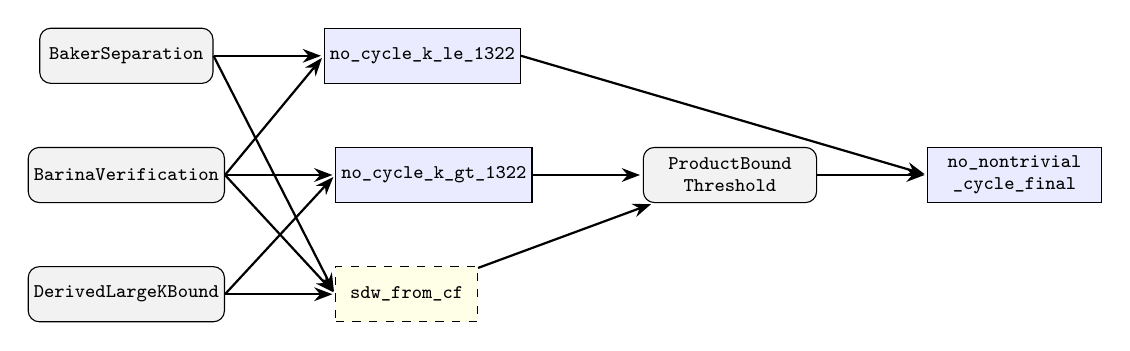
\begin{tikzpicture}[
  node distance=8mm and 10mm,
  hyp/.style={rectangle, draw, rounded corners, fill=gray!10,
              align=center, font=\scriptsize\ttfamily,
              minimum height=7mm, minimum width=22mm,
              inner sep=2pt},
  thm/.style={rectangle, draw, fill=blue!8, align=center,
              font=\scriptsize\ttfamily, minimum height=7mm,
              minimum width=22mm, inner sep=2pt},
  bridge/.style={rectangle, draw, dashed, fill=yellow!10,
                 align=center, font=\scriptsize\ttfamily,
                 minimum height=7mm, minimum width=18mm,
                 inner sep=2pt},
  arr/.style={->, >=Stealth, thick, shorten >=1pt}
]
\node[hyp] (B) {BakerSeparation};
\node[hyp, below=of B] (Ba) {BarinaVerification};
\node[hyp, below=of Ba] (D) {DerivedLargeKBound};

\node[thm, right=14mm of B] (kle) {no\_cycle\_k\_le\_1322};
\node[thm, right=14mm of Ba] (kgt) {no\_cycle\_k\_gt\_1322};
\node[bridge, right=14mm of D] (sdw) {sdw\_from\_cf};

\node[hyp, right=14mm of kgt] (PBT) {ProductBound\\Threshold};

\node[thm, right=14mm of PBT] (final) {no\_nontrivial\\\_cycle\_final};

\draw[arr] (B) -- (kle);
\draw[arr] (Ba.east) -- (kle.west);
\draw[arr] (Ba) -- (kgt);
\draw[arr] (D.east) -- (kgt.west);
\draw[arr] (B.east) -- (sdw.west);
\draw[arr] (Ba.east) -- (sdw.west);
\draw[arr] (D) -- (sdw);
\draw[arr] (sdw) -- (PBT);
\draw[arr] (kle.east) -- (final.west);
\draw[arr] (kgt.east) -- (PBT.west);
\draw[arr] (PBT) -- (final);
\end{tikzpicture}}
\caption{Dependency graph of the seven central theorems.
Hypothesis structures (gray) feed the two sub-branch theorems
(blue, $k \leq 1322$ and $k > 1322$) and the bridge lemma
\texttt{sdw\_from\_cf} (yellow, dashed); the canonical theorem
\texttt{no\_nontrivial\_cycle\_final} sits at the right. The
bridge lemma converts \texttt{DerivedLargeKBound} into
\texttt{ProductBoundThreshold} under the standard hypotheses,
making the two formulations interderivable.}
\label{fig:depgraph}
\end{figure}

\subsection{Infrastructure lemmas (continued-fraction
side)}\label{infrastructure-lemmas-continued-fraction-side}

Three dedicated modules formalize the classical continued-fraction
theory needed by §7 and by the Phase59 sub-branch
\texttt{no\_cycle\_k\_gt\_1322}:

\begin{itemize}
\tightlist
\item
  \textbf{\texttt{ProjetCollatz/Phase60IrrationalityLog23.lean}} ---
  irrationality of \texttt{log\_2\ 3} and the corollary
  \texttt{2\^{}s\ ≠\ 3\^{}k} for all \texttt{(s,\ k)} with
  \texttt{k\ ≥\ 1} (used in the product-bound obstruction reasoning of
  §5).
\item
  \textbf{\texttt{ProjetCollatz/Phase61CFConvergents.lean}} ---
  convergents \texttt{Real.convergent\ log\_2\ 3\ n}, the denominators
  \texttt{q\_n}, the window predicate
  \texttt{InWindow\ n\ k\ ↔\ q\_n\ ≤\ k\ \textless{}\ q\_\{n+1\}}, the
  bridge theorem
  \texttt{q\_n\_eq\_den:\ (Real.convergent\ log\_2\ 3\ n).den\ =\ q\_n},
  and the far-approximation lemma
  \texttt{not\_convergent\_implies\_far\_approx}.
\item
  \textbf{\texttt{ProjetCollatz/Phase62BestApproxBridge.lean}} --- the
  public approximation bound \texttt{log23\_abs\_sub\_convergent\_le},
  its parametric in-window variant
  \texttt{log23\_abs\_sub\_convergent\_le\_in\_window}, the wrapper
  \texttt{of\_convs\_eq\_log23\_convergent}, and non-termination of the
  continued-fraction expansion \texttt{log23\_never\_terminates}.
\end{itemize}

These continued-fraction infrastructure theorems have axiom profile
\texttt{{[}propext,\ Classical.choice,\ Quot.sound{]}} --- the three
standard Mathlib kernel axioms, no more. They are not in the central
chain of \texttt{no\_nontrivial\_cycle\_final} (which goes via Phase58
directly); they are in the central chain of the variant
\texttt{no\_nontrivial\_cycle\_phase59} via
\texttt{no\_cycle\_k\_gt\_1322}.

\subsection{\texorpdfstring{Arithmetic gap constants verified by
\texttt{native\_decide}}{Arithmetic gap constants verified by native\_decide}}\label{arithmetic-gap-constants-verified-by-native_decide}

Six windows \texttt{W\_8,\ ...,\ W\_\{13\}} of continued-fraction
denominators of \texttt{log\_2\ 3} (see §2.5 for numerical values) come
with six ``gap constants'' \texttt{cf\_gap\_n:\ ℕ} and six window-size
bounds \texttt{cf\_nbound\_n:\ ℕ}, all proved by Lean's
\texttt{native\_decide} tactic in
\texttt{ProjetCollatz/Phase59ContinuedFractions.lean}. Three of these
are sampled in the probe \texttt{probes/check\_central\_axioms.lean}
(\texttt{cf\_gap\_8}, \texttt{cf\_gap\_13}, \texttt{cf\_nbound\_8});
their axiom profile is
\texttt{{[}propext,\ Lean.ofReduceBool,\ Lean.trustCompiler{]}} --- the
three standard \texttt{native\_decide} axioms, and nothing else.

These twelve arithmetic lemmas are \textbf{isolated from the central
chain} at the current formalization state: they are consumed only
through \texttt{sdw\_from\_cf} (§8.1 table), which is itself called only
through \texttt{no\_nontrivial\_cycle\_phase59}, not through
\texttt{no\_nontrivial\_cycle\_final}. The isolation is recorded in
\texttt{expected\_axioms.md} (§8.6) and enforced by
\texttt{reproduce.sh} (§8.7). It is also the reason why the central
chain of \texttt{no\_nontrivial\_cycle\_final} is kernel-3, despite the
presence of the \texttt{native\_decide} axioms elsewhere in the project.

A forthcoming pass on the Phase63 skeleton (§8.4) would integrate the
gap constants directly into the central chain; such a pass is
structurally blocked by the obstruction of §5.

\subsection{The Phase63 skeleton}\label{the-phase63-skeleton}

The file \texttt{ProjetCollatz/Phase63DerivedLargeKBoundTheorem.lean}
(175 lines, \textbf{Section 1 only}, no \texttt{theorem} /
\texttt{lemma} declarations) preserves, as a documented skeleton, the
architecture that would be needed to promote the Phase59 structure
\texttt{DerivedLargeKBound} from hypothesis to theorem. Its Section 1
consists of:

\begin{itemize}
\tightlist
\item
  Imports (2 Mathlib + 5 Phase58-62 transitive dependencies);
\item
  Namespace \texttt{ProjetCollatz.Phase63} and \texttt{open}
  declarations for the 12 arithmetic constants \texttt{cf\_gap\_8..13}
  and \texttt{cf\_nbound\_8..13};
\item
  A detailed module docstring laying out the eleven-section architecture
  originally planned;
\item
  A footer added at Commit \#1 (\texttt{d41e2e9}) explicitly recording
  that Sections 2-11 are \textbf{not implemented} and redirecting to §5
  (Obstruction I) of this paper for the structural reason.
\end{itemize}

The skeleton is kept in the repository so that future readers trace the
original design; it \textbf{does not participate} in the central chain
of \texttt{no\_nontrivial\_cycle\_final} or any of its aliases. The
axiom profile of the file (as a whole) is vacuous --- no theorem is
declared.

\subsection{Structural-excess framework (extension, separate
branch)}\label{structural-excess-framework-extension-separate-branch}

Alongside the main formalization described above, a parallel Lean 4
effort develops a custom \emph{structural-excess} framework
\texttt{Φ\_s\ /\ Ψ\_s} for quantifying deviations of cycle parity
vectors from an i.i.d.-Bernoulli null, motivated by the probabilistic
discussion of §9. Because Mathlib v4.27.0 lacks a native Gowers-norm
library, this framework is implemented from first principles in a
dedicated module \texttt{ProjetCollatz/PhaseVIII/StructuralExcess.lean}.

The extension is provided as the supplementary \texttt{PhaseVIII/}
sub-directory of the accompanying repository. It is \textbf{not} part of
the central proof chain that carries this paper's main theorem and its
kernel-3 axiom profile verification; it sits alongside, with a clearly
separated namespace and probe.

The extension contains: parametric definitions of \(\Phi_s\) and
\(\Psi_s\); a machine-verified evaluation of the trivial Collatz cycle
as \texttt{trivialCycle\_psi2:\ ...\ =\ 32/81\ :=\ by\ native\_decide},
establishing a concrete non-zero structural excess on the unique known
cycle of the \(3x+1\) map; a parametric \texttt{Prop} definition for the
T4c conjecture of §9; a contradiction schema
\texttt{psi2\_bounds\_no\_cycle} showing how a future T4c proof would
discharge the cycle problem; and an axiom-audit probe confirming
\textbf{zero new user axioms}, which leaves the extension's axiom
profile at the standard kernel three plus the two
\texttt{native\_decide} axioms inherited from the one
\texttt{trivialCycle\_psi2} evaluation.

Nothing in §1-§7 depends on the \texttt{PhaseVIII/} extension; its
status is purely supplementary. The reader interested in the
structural-excess viewpoint is referred to §9 for the mathematical
framing and to \texttt{ProjetCollatz/PhaseVIII/} for the Lean source.

\subsection{\texorpdfstring{Expected axiom profile
(\texttt{expected\_axioms.md})}{Expected axiom profile (expected\_axioms.md)}}\label{expected-axiom-profile-expected_axioms.md}

The project publishes a reference snapshot of the
\texttt{\#print\ axioms} baseline at the repository root, file
\texttt{expected\_axioms.md}. Its Section 1 lists the \emph{central}
theorems (as in §8.1) with expected axiom set
\texttt{{[}propext,\ Classical.choice,\ Quot.sound{]}}. Its Section 2
lists three sampled auxiliary \texttt{native\_decide} lemmas with
expected set
\texttt{{[}propext,\ Lean.ofReduceBool,\ Lean.trustCompiler{]}}. The
remaining sections document the out-of-scope structures and the
forbidden-axiom patterns enforced by the probe.

The baseline is enforced by the probe
\texttt{probes/check\_central\_axioms.lean} (plus the dedicated
Phase-level probes \texttt{check\_phase60..63\_axioms.lean}), and any
deviation triggers a non-zero exit from \texttt{reproduce.sh}.

\subsection{\texorpdfstring{Reproducibility
(\texttt{reproduce.sh})}{Reproducibility (reproduce.sh)}}\label{reproducibility-reproduce.sh}

A single shell script at the repository root encapsulates the full
verification pipeline:

\begin{Shaded}
\begin{Highlighting}[]
\FunctionTok{bash}\NormalTok{ reproduce.sh}
\CommentTok{\# 0: all checks PASS}
\CommentTok{\# 1: toolchain mismatch (lean{-}toolchain / elan)}
\CommentTok{\# 2: Lean build error or sorry{-}related warning}
\CommentTok{\# 3: axiom drift (unexpected or missing axiom vs expected\_axioms.md)}
\CommentTok{\# 4: sorryAx detected in the central or auxiliary chain}
\end{Highlighting}
\end{Shaded}

The five steps of the script are (i) toolchain check, (ii) Mathlib cache
fetch, (iii) \texttt{lake\ build\ ProjetCollatz}, (iv) axiom probe on
\textbf{25 theorems} (7 central + 3 auxiliary + 15 M3 foundational), and
(v) sorry probe. On a fresh clone with cache available, the total
runtime is of the order of 3-5 minutes (incremental: 10 seconds); on a
from-source build without cache, of the order of 90 minutes. The
Continuous-Integration workflow at \texttt{.github/workflows/verify.yml}
runs the same checks on every push and pull-request.

\subsection{Integrity invariants}\label{integrity-invariants}

The following project-wide invariants are enforced by the combination of
the probes, \texttt{reproduce.sh}, and the project's review protocol:

\begin{itemize}
\tightlist
\item
  \textbf{No user \texttt{axiom} declaration.} No file in
  \texttt{ProjetCollatz/} introduces a new axiom; the only axioms in the
  transitive closure are the Mathlib kernel axioms listed in §8.6.
\item
  \textbf{No \texttt{sorry}, \texttt{admit}, or \texttt{stop}.} Every
  declaration has a complete proof term; the \texttt{sorryAx} probe
  (\texttt{probes/check\_sorry.lean}) is run as a separate step by
  \texttt{reproduce.sh} for defense in depth.
\item
  \textbf{All docstrings are in English.}
\end{itemize}

These are enforced per-commit and recorded in the project's development
journal.

\section{Open problems}\label{open-problems}

\subsection{\texorpdfstring{Removing
\texttt{ProductBoundThreshold}}{Removing ProductBoundThreshold}}\label{removing-productboundthreshold}

The central open question raised by this paper: can
\texttt{ProductBoundThreshold} be promoted to a theorem? §5 Obstruction
I answers \emph{not within any product-bound approach}. The question is
therefore: what non-product-bound technique might close the
\texttt{k\ \textgreater{}\ 1322} case?

\subsection{\texorpdfstring{The \texttt{k\ ≥\ q\_\{14\}}
tail}{The k ≥ q\_\{14\} tail}}\label{the-k-q_14-tail}

Current-generation Barina reaches \texttt{n\ \textless{}\ 2\^{}\{71\}},
which via CF windows \texttt{W\_8,\ ...,\ W\_\{13\}} covers
\texttt{k\ \textless{}\ q\_\{14\}\ ≈\ 10,590,737}. A \texttt{W\_\{14\}}
extension would require arithmetic gap constants involving
\texttt{3\^{}\{q\_\{14\}\}}, a number with approximately
\texttt{5\ ·\ 10\^{}6} decimal digits --- outside
\texttt{native\_decide}'s reach at present hardware.

\subsection{Formalization challenges}\label{formalization-challenges}

\begin{itemize}
\tightlist
\item
  The bridge
  \texttt{(Real.convergent\ v\ n).den:\ ℝ\ =\ (GenContFract.of\ v).dens\ n}
  is not direct in Mathlib v4.27.0. Phase62 works around it via a
  parametric real-valued form; a proper bridge would strengthen the
  Phase61 / Phase62 integration.
\item
  Phase63 Sections 2-11 as Lean theorems would require the breakthrough
  discussed in §9.1 + the bridge in §9.3.
\end{itemize}

\subsection{Relation to divergence}\label{relation-to-divergence}

This paper does not address the divergence half of Collatz. The
techniques (Baker's theorem + CF theory + formal verification) are in
principle adaptable, but the structure is different. Explicit scope
disclosure.

\subsection{Speculative tracks
pointer}\label{speculative-tracks-pointer}

Ongoing speculative investigations on transcendence-theoretic approaches
(Santana 2026 rigor-closure, Knight 2026 extension, transcendence-gap
sharpenings). Results, if any, would feed a future paper revision.

\subsection{Probabilistic techniques
(Tao)}\label{probabilistic-techniques-tao}

Tao's probabilistic approach (2019, \emph{Forum of Mathematics, Pi})
proves that almost all Collatz orbits attain almost bounded values under
logarithmic density. This result is \textbf{probabilistic} and does not
extend to deterministic statements about hypothetical cycles (which have
density zero). Tao's broader toolkit (entropy compression à la
Moser-Tardos {[}blog 2009{]}, higher-order Fourier analysis à la
Green-Tao-Ziegler) has not been successfully applied to deterministic
Collatz cycle bounds; such applications would require substantial new
theoretical work. We therefore do not integrate probabilistic techniques
into our proof of Theorem 3.1 (which remains conditional on the
structural hypotheses §4).

\subsection{Structural-excess framework
Ψ\_s}\label{structural-excess-framework-ux3c8_s}

\emph{{[}Lean formalization status: see §8.5 for the supplementary
\texttt{ProjetCollatz/PhaseVIII/} module.{]}}

We formalize in Lean 4 a custom \(\Phi_s / \Psi_s\) structural-excess
framework (Mathlib v4.27.0 lacks Gowers norms). Machine-verified: the
trivial Collatz cycle has \(\Psi_2 = 32/81\), establishing a
factor-\(32\times\) structural excess over its mean prediction
(\(1/81\)). The T4c conjecture is encoded as parametric
\texttt{def\ T4c\_Conjecture\_Psi2}, and the contradiction schema
\texttt{psi2\_bounds\_no\_cycle} records the logical shape of the
intended attack. See \texttt{ProjetCollatz.PhaseVIII.StructuralExcess}
in the accompanying repository (§8.5).

\subsection{Set-theoretic and rigidity-based research
directions}\label{set-theoretic-and-rigidity-based-research-directions}

\textbf{Status note.} The remainder of this section sketches a
research-direction frame --- not a result. None of the constructions
below participates in the central proof chain of §3, none is formalized
in the kernel-3 Lean baseline, and none is asserted as established
mathematics. We include the sketch here for transparency about the lines
of work the present paper does \emph{not} close, and as forward pointers
to Appendix A where the alternate-notation explorations are gathered.

The frame, inherited from the Hercher / Steiner cycle-structure
literature, uses the alternate notation of Appendix A (\(a\) = even
steps, \(k\) = odd steps, \(T = a + k\) the cycle period,
\(q = 2^a - 3^k\) the Steiner difference, \(K\) for Hercher's
cycle-length invariant per §6.1 note, \(R_K(\sigma) := \sum_i
3^{K-1-i} \cdot 2^{\sigma(i)}\) for the permutation sum behind the
Steiner rigidity question, and \(\psi_s, \Psi_s\) for the
structural-excess functions of §9.7).

The frame organizes a hypothetical cycle's parity vector as sitting
inside an intersection
\(S_{\mathrm{cycle}} \subset S_{\mathrm{Steiner}} \cap
S_{\Psi\text{-large}} \cap S_{\mathrm{Kol\text{-}bounded}} \setminus
S_{\mathrm{Hercher}}\) --- combining Steiner-rigid tuples, a
\(\Psi_s\)-excess condition (cf.~§9.7), and a conditional-Kolmogorov
compressibility condition. Five ``bricks'' \(W_1, W_2, W_3, W_4, W_5\)
of this frame are exploited or reduced to redundancy in the present
paper, except for \(W_2\) (Steiner rigidity), which is the remaining
open input. We refer to this informally as the \emph{Wall DNA}
arrangement and to its conjectural closure as the \emph{META-ROADMAP}
statement; both labels are descriptive shorthand, not theorems. A
200-line exploratory Lean 4 prototype attaches a \texttt{sorry}
placeholder to the META-ROADMAP statement under five hypotheses
(\texttt{hSteinerRigidity}, \texttt{hCycle}, \texttt{hPsiLarge},
\texttt{hKolBounded}, \texttt{hHercher}); the only machine-verified part
of the prototype is the trivial-cycle evaluation \(\psi_2 = 32/81\),
reusing the structural-excess framework of §8.5. \textbf{None of this
prototype lies in the central chain of
\texttt{no\_nontrivial\_cycle\_final}, none of its hypotheses is proven,
and the present paper does not claim that any such closure is
achievable.}

A boundary scan over classical mechanisms (Schmidt subspace theorems for
transcendental \(\alpha\), Tao 2019/2022 entropy compression for typical
orbits, Lagarias's \(T_\infty\) Galton--Watson framework) confirms that
none extends to deterministic cycle bounds without substantial
additional work. Salikhov 2007 combined with Hercher 2023, in this
alternate notation, yields a \(q \gg 2.836^k\) lower bound (Proposition
A.1) under the explicit conditioning of Appendix A. These extensions are
documented in \textbf{Appendix A} with self-contained notation; we
reference them here only as forward pointers.

\section{Conclusion}\label{conclusion}

This paper presents a machine-checked conditional non-existence result
for non-trivial Collatz cycles, three named hypotheses on which it
rests, two impossibility lemmas explaining why the third hypothesis
cannot be discharged within the standard Diophantine framework, and a
literature mapping documenting the structural gap that makes the
conditionality necessary. The Lean 4 formalization is reproducible under
Mathlib v4.27.0 with an isolated and documented axiom profile.

\subsection{What this paper
establishes}\label{what-this-paper-establishes}

The five contributions of §1.3 are realized as follows:

\begin{itemize}
\item
  \textbf{6α (formal verification, §3 + §8).} The conditional theorem
  \texttt{no\_nontrivial\_cycle\_final}
  (\texttt{ProjetCollatz/Phase58PorteDeuxFinal.lean} line 339) is
  declared parametrically with the three structures of §4 and is
  machine-verified. Its kernel-3 axiom profile (\texttt{propext},
  \texttt{Classical.choice}, \texttt{Quot.sound}) is exhibited verbatim
  in §3.3 and §8.6, and reproducibility is encoded in
  \texttt{reproduce.sh} against the \texttt{expected\_axioms.md}
  baseline (§8.7).
\item
  \textbf{\(\delta 7\) (alternative framing, §7).} Reformulation
  \ref{ref:disjunction} restates the central result equivalently as the
  disjunction ``\(k \leq 1322\) or \(n > 2^{71}\)'' (§7.1), establishing
  a one-sentence bridge from the conditional theorem to Hercher's (2023)
  lower bound \(K > 1.375 \cdot 10^{11}\) (§7.2). A finer-grained
  continued-fraction refinement at the cycle-length scale \(k > 1322\)
  is documented as a Phase63 Lean skeleton (§8); its non-completion
  meets the obstruction of §5.
\item
  \textbf{\(\delta 8\) (Product-Bound Impossibility Lemma, §5.1).} Lemma
  \ref{lem:productbound} formalizes a meta-mathematical obstruction:
  every uniform algebraic bound \(F(k)\) with \(F(k) < 2^{71}\) derived
  through the Product Bound derivation forces an irrationality-measure
  constraint on \(\log_2 3\) that contradicts irrationality. The lemma
  is a publication-only argument about the structural limits of the
  Baker + continued- fraction framework, not a Lean theorem.
\item
  \textbf{\(\delta 8'\) (extended impossibility, §5.2).} Corollary
  \ref{cor:lowerasymmetry} extends \(\delta 8\) to Baker-type
  inequalities composed with Steiner's cycle equation. Window-by-window
  numerical corroboration via Khinchin's best-second-kind
  characterization closes \(k \leq 982\) (Baker \(\mu = 6\)),
  \(k \leq 3693\) (Salikhov 2007 \(\mu = 5.125\)), and
  \(k \lesssim 3 \cdot 10^{10}\) (Khinchin per-window) --- all below
  Hercher's lower bound \(K > 1.375 \cdot 10^{11}\).
\item
  \textbf{\(\delta 9\) (state-of-the-art mapping, §6).} Section 6
  catalogs the 1977-2026 Collatz cycle literature in five categories:
  historical lower bounds (§6.1), structural-class eliminations (§6.2),
  meta-impossibilities (§6.3), recent reformulation attempts (§6.4), and
  probabilistic / density results (§6.5). The mapping documents, to the
  best of our literature review, the absence of any peer-reviewed
  deterministic upper bound on cycle length \(k\) for general Collatz
  cycles (§6.6).
\end{itemize}

\subsection{What this paper does not
claim}\label{what-this-paper-does-not-claim}

\begin{itemize}
\item
  We do \textbf{not} prove the Collatz conjecture. The third hypothesis,
  \texttt{ProductBoundThreshold} (§4.3), remains a hypothesis; the paper
  is \emph{about} why it cannot be discharged within the standard
  framework.
\item
  We do \textbf{not} address the divergence half of the Collatz
  conjecture (§1.1). The cycle problem and the divergence problem are
  disjoint; this paper concerns only the former.
\item
  We do \textbf{not} dismiss or subsume Santana (2026), Knight (2026),
  Dhiman-Pandey (2026), or Rozier-Terracol (2026). Each is situated in
  §6.4 as either complementary (different methodological framework) or
  restricted-class (does not extend to general cycles), with the
  documented gaps and indirect-source flags clearly attributed.
\item
  We do \textbf{not} claim that the obstruction of §5 is final. The
  obstruction is structural under the \emph{Baker + CF + Product Bound}
  paradigm; methodological frameworks outside that paradigm --- for
  instance a deterministic upper bound on cycle length derived from
  ergodic, density-theoretic, or yet-uncataloged techniques --- would
  immediately discharge \texttt{ProductBoundThreshold} and upgrade
  Theorem \ref{thm:main} from conditional to unconditional.
\end{itemize}

\subsection{Modular invitation for future
work}\label{modular-invitation-for-future-work}

The paper's structure is deliberately additive: conditional theorem +
documented obstructions + machine-verifiable formalization. A future
contribution that resolves any of the three following lines of work
would, without further editorial intervention, upgrade the conditional
theorem:

\begin{enumerate}
\def\labelenumi{\arabic{enumi}.}
\item
  \textbf{Discharge \texttt{ProductBoundThreshold}} (§4.3). Any
  deterministic proof that hypothetical cycles satisfy \(k \leq K\) for
  some explicit \(K\) (whether \(K = 982\) or larger) would replace the
  structure field with a Lean theorem.
\item
  \textbf{Close the \(\delta 9\) gap} (§6.6). A peer-reviewed
  deterministic upper bound on \(k\) for general cycles, by any
  methodological framework, would supersede the project-specific
  encoding.
\item
  \textbf{Refine or supersede \(\delta 8\)} (§5). A novel argument
  framework not bound by the Baker + CF + Product Bound family of
  inequalities could in principle bypass the obstruction, with
  corresponding refinement of the conditional theorem.
\end{enumerate}

Speculative tracks documented in §9 (open problems) --- including the
\(\Psi_s\) structural-excess framework (§9.7) and the upper-bound
complement attempt (§9.8) --- are presented as ongoing work not
integrated into the central conditional theorem of §3; we list them for
transparency and as invitations rather than as results.

The Lean 4 formalization is intended as a stable substrate for such
future work: the conditional theorem, the three hypothesis structures,
and the axiom profile are all parametric, so additive contributions need
not re-formalize the existing argument.

\subsection*{Data and code
availability}\label{data-and-code-availability}
\addcontentsline{toc}{subsection}{Data and code availability}

All paper sources, the Lean 4 formalization, the verification probes,
and the reproduction script are publicly available at
\url{https://github.com/ericmerle3789/collatz-conditional-cycles}
(branch \texttt{main}; the release commit hash will be recorded in the
Zenodo metadata upon deposit). Reproduction requires the Lean toolchain
\texttt{leanprover/lean4:v4.27.0} against Mathlib commit
\texttt{a3a10db0e9d66acbebf76c5e6a135066525ac900} (pinned in the
project's \texttt{lake-manifest.json}). With the Mathlib cache fetched,
full reproduction completes in approximately 5 minutes on a Mac M1 Pro
with 16 GB RAM, exiting with kernel-3 axiom profile and zero
\texttt{sorry}. The exit-code semantics of \texttt{reproduce.sh} (0 =
success, 1 = toolchain mismatch, 2 = build failure, 3 = axiom drift, 4 =
\texttt{sorryAx} detected) are documented in §8.7.

\subsection*{Acknowledgements}\label{acknowledgements}
\addcontentsline{toc}{subsection}{Acknowledgements}

The Lean formalization builds on Mathlib (Mathematics in Lean 4); the
author thanks the Mathlib community for the continued-fraction,
Diophantine-approximation, and number-theory infrastructure on which the
central chain depends. The author also thanks D. Barina for the 2025
computational verification underpinning hypothesis (ii). The
state-of-the-art mapping in §6 is indebted to the cumulative work of the
Collatz literature 1977-2026 surveyed therein.

The author used Claude Opus 4.7 (Anthropic) during manuscript
preparation for drafting, revision, and literature retrieval, and Lean 4
(the proof assistant) for the machine-verification of the central
theorem chain. The mathematical content and the scientific
responsibility for the manuscript rest with the author; the formal
verification is mechanically checked under the standard kernel-3 axiom
profile (\texttt{propext}, \texttt{Classical.choice},
\texttt{Quot.sound}), as documented in §8.6 and Appendix B, and is
therefore independent of the assistance described above.

\section{References}\label{references}

\subsection*{Peer-reviewed}\label{peer-reviewed}
\addcontentsline{toc}{subsection}{Peer-reviewed}

\begin{enumerate}
\def\labelenumi{\arabic{enumi}.}
\tightlist
\item
  A. Baker, \emph{Linear forms in the logarithms of algebraic numbers
  I}, Mathematika 13 (1966), 204-216.
\item
  R. Terras, \emph{A stopping time problem on the positive integers},
  Acta Arithmetica 30 (1976), 241-252.
\item
  R. P. Steiner, \emph{A theorem on the Syracuse problem}, in
  \emph{Proceedings of the 7th Manitoba Conference on Numerical
  Mathematics}, Utilitas Mathematica Publishing, Winnipeg, MB, 1977,
  pp.~553-559.
\item
  R. E. Crandall, \emph{On the ``3x+1'' problem}, Mathematics of
  Computation 32 (1978), 1281-1292.
\item
  A. Ya. Khinchin, \emph{Continued Fractions}, Dover Publications, 1997
  (reprint of the 1964 University of Chicago Press translation). ISBN
  978-0-486-69630-0.
\item
  J. C. Lagarias, \emph{The 3x+1 problem and its generalizations},
  American Mathematical Monthly 92 (1985), 3-23. DOI: 10.2307/2322189.
\item
  D. Applegate and J. C. Lagarias, \emph{Density bounds for the 3x+1
  problem. I. Tree-search method}, Mathematics of Computation 64 (1995),
  no. 209, 411-426; \emph{Density bounds for the 3x+1 problem. II.
  Krasikov inequalities}, Mathematics of Computation 64 (1995), no. 209,
  427-438.
\item
  G. Rhin, \emph{Approximants de Padé et mesures effectives
  d'irrationalité}, in \emph{Séminaire de Théorie des Nombres, Paris
  1985-86} (C. Goldstein, ed.), Progress in Mathematics 71, Birkhäuser,
  Boston, MA, 1987, pp.~155-164. DOI: 10.1007/978-1-4757-4267-1\_11.
\item
  V. Kh. Salikhov, \emph{On the irrationality measure of ln 3}, Doklady
  Mathematics 76 (2007), no. 3, 955-957. DOI: 10.1134/S1064562407060361.
\item
  Q. Wu, \emph{On the linear independence measure of logarithms of
  rational numbers}, Mathematics of Computation 72 (2003), no. 242,
  901-911. DOI: 10.1090/S0025-5718-02-01442-4.
\item
  E. M. Matveev, \emph{An explicit lower bound for a homogeneous
  rational linear form in the logarithms of algebraic numbers. II},
  Izvestiya: Mathematics 64 (2000), no. 6, 1217-1269. DOI:
  10.1070/IM2000v064n06ABEH000314.
\item
  J. L. Simons and B. M. M. de Weger, \emph{Theoretical and
  computational bounds for m-cycles of the 3n+1 problem}, Acta
  Arithmetica 117 (2005), 51-70. DOI: 10.4064/aa117-1-3.
\item
  S. Eliahou, \emph{The 3x+1 problem: new lower bounds on nontrivial
  cycle lengths}, Discrete Mathematics 118 (1993), no. 1-3, 45-56. DOI:
  10.1016/0012-365X(93)90052-U.
\item
  I. Krasikov and J. C. Lagarias, \emph{Bounds for the 3x+1 problem
  using difference inequalities}, Acta Arithmetica 109 (2003), 237-258.
  DOI: 10.4064/aa109-3-4.
\item
  J. C. Lagarias, editor, \emph{The Ultimate Challenge: The 3x+1
  Problem}, AMS, 2010. ISBN 978-0-8218-4940-8.
\item
  T. Tao, \emph{Almost all orbits of the Collatz map attain almost
  bounded values}, Forum of Mathematics, Pi 10 (2022), e12,
  arXiv:1909.03562 (2019). DOI: 10.1017/fmp.2022.8.
\item
  D. Barina, \emph{Improved verification limit for the convergence of
  the Collatz conjecture}, J. Supercomp. 81 (2025), no. 7, 810. DOI:
  10.1007/s11227-025-07337-0.
\item
  C. Hercher, \emph{There are no Collatz m-Cycles with m ≤ 91}, J.
  Integer Seq. 26 (2023), Article 23.3.5.
  \url{https://cs.uwaterloo.ca/journals/JIS/VOL26/Hercher/hercher5.html}.
\item
  K. Knight, \emph{Collatz high cycles do not exist}, Discrete
  Mathematics 349 (2026), no. 3, 114812. DOI:
  10.1016/j.disc.2025.114812. \emph{(Cited indirectly: full PDF access
  was not available at the time of writing; we rely on the published
  abstract and on cumulative-literature attribution. See §6.2.)}
\end{enumerate}

\subsection*{Preprints (cited with
disclosure)}\label{preprints-cited-with-disclosure}
\addcontentsline{toc}{subsection}{Preprints (cited with disclosure)}

\begin{enumerate}
\def\labelenumi{\arabic{enumi}.}
\setcounter{enumi}{19}
\tightlist
\item
  E. Santana, \emph{On the Collatz Conjecture: Topological and Ergodic
  Approach}, arXiv:2601.03297v4 (2026).
\item
  B. Honarvar Shakibaei Asli, \emph{An Explicit Near-Conjugacy Between
  the Collatz Map and a Circle Rotation}, arXiv:2601.04289 (2026).
\item
  O. Rozier and C. Terracol, \emph{Paradoxical behavior in Collatz
  sequences}, arXiv:2502.00948 (2025), to appear in \emph{Discrete
  Mathematics} 349, 115167 (2026).
\item
  M. Dhiman and R. Pandey, \emph{2-Adic Obstructions to
  Presburger-Definable Characterizations of Collatz Cycles},
  arXiv:2601.12772 (2026).
\end{enumerate}

\subsection*{Software and data}\label{software-and-data}
\addcontentsline{toc}{subsection}{Software and data}

\begin{enumerate}
\def\labelenumi{\arabic{enumi}.}
\setcounter{enumi}{23}
\tightlist
\item
  The Mathlib Community, \emph{The Lean Mathematical Library}, v4.27.0
  (2026). \url{https://leanprover-community.github.io/mathlib4/}
\item
  E. Merle, \emph{collatz-conditional-cycles}, repository accompanying
  this paper.
  \url{https://github.com/ericmerle3789/collatz-conditional-cycles}
  (branch \texttt{main}, at the release commit recorded in the Zenodo
  metadata).
\end{enumerate}

\appendix

\section{Alternate-notation explorations of the high-complexity
disjunct}\label{alternate-notation-explorations-of-the-high-complexity-disjunct}

This appendix builds on the META-ROADMAP THEOREM framing of §9.8.3 (Wall
DNA Theorem, brick \(W_2\)) and the Lean prototype of §9.8.5 (documented
in the accompanying repository). It isolates the alternate-notation
results that use a convention inherited from the Hercher 2023 / Steiner
cycle-structure literature. Throughout the appendix we adopt this
paper's \((a, k)\) convention (consistent with §3 and §4): \(a\) is the
number of even steps in a hypothetical cycle, \(k\) is the number of odd
steps, and \(q := 2^a - 3^k\) is the Steiner difference. Where Hercher
2023 writes \(K\) for the number of odd elements in a cycle (cf.~Theorem
27 of \emph{op. cit.} and §6.1 above), we have \(K = k\); where Hercher
writes \(T\) for the cycle period, we have \(T = a + k\). The appendix
is otherwise self-contained.

\subsection{\texorpdfstring{Salikhov 2007 + Hercher 2023 establish a
\(q \gg 2.836^k\) lower
bound}{Salikhov 2007 + Hercher 2023 establish a q \textbackslash gg 2.836\^{}k lower bound}}\label{salikhov-2007-hercher-2023-establish-a-q-gg-2.836k-lower-bound}

\begin{proposition}[Conditional consequence of Salikhov 2007 and Hercher 2023]
\label{thm:Aone}
\emph{Conditional on (i) Hercher's Corollary 29 lower bound
$K > 1.375 \cdot 10^{11}$, (ii) Salikhov's irrationality-measure
result $\mu(\ln 3) \leq 5.125$, and (iii) an effective
linear-form lemma turning (ii) into}
$|p \cdot \ln 2 - k \cdot \ln 3| \geq C_{\ln} / k^c$
\emph{with} $c \leq 5.125$, $C_{\ln} > 0$, \emph{and $k$ above an
effective threshold $k_0$ — none of which is established here} —
\emph{for every admissible Collatz cycle $(a, k)$, with $a$ and
$k$ related by} $a = \lceil k \cdot \log_2 3 \rceil$
\emph{(so that} $2^a > 3^k > 2^{a-1}$\emph{) and with}
$k > 1.375 \cdot 10^{11}$,
$$
q := 2^a - 3^k > 2.836^k.
$$
\end{proposition}

\textbf{Proof sketch.} Set \(\alpha = k \cdot \log_2 3\) and write
\(a = \lceil \alpha \rceil\), so \(0 < a - \alpha \leq 1\). Since
\(3^k = 2^{\alpha}\), the Steiner difference satisfies
\(q = 2^a - 3^k = 3^k \cdot (2^{a - \alpha} - 1)\). Using the elementary
inequality \(2^x - 1 \geq x \cdot \ln 2\), valid for \(x \in (0, 1]\),
we obtain \(q \geq 3^k \cdot (a - \alpha) \cdot \ln 2\). The effective
irrationality measure \(\mu(\ln 3) \leq 5.125\) (Salikhov 2007, refining
Rhin 1987's linear-form bound \(\leq 8.616\)) yields, in linear-form
shape, \(|p \cdot \ln 2 - k \cdot \ln 3| \geq C_{\ln} / k^c\) for
\(c \leq 5.125\), an effective constant \(C_{\ln} > 0\), and \(k\)
sufficiently large. Translating to the \(\log_2 3\) form via
\(\log_2 3 = \ln 3 / \ln 2\) gives
\(a - \alpha = a - k \cdot \log_2 3 \geq C \cdot k^{-(c-1)}\) with
\(C = C_{\ln} / \ln 2\); for \(c = 5.125\) this is the bound
\(a - \alpha \geq C \cdot k^{-4.125}\). Combining:
\(q \geq C \cdot \ln 2 \cdot 3^k \cdot k^{-4.125}\). The conclusion
\(q > 2.836^k\) then reduces to
\((3/2.836)^k > k^{4.125} / (C \cdot \ln 2)\). Since
\(\log_2(3/2.836) \approx 0.0811 > 0\), the left-hand side grows
exponentially in \(k\) while the right-hand side grows polynomially;
under Hercher's lower bound \(k > 1.375 \cdot 10^{11}\) the inequality
holds with an enormous margin (the exponential side is approximately
\(10^{3.4 \cdot 10^9}\), dwarfing any polynomial in \(k\)), and the
threshold \(k_0\) from Salikhov's effective bound sits well below
\(1.375 \cdot 10^{11}\). Theorem \ref{thm:Aone} therefore establishes
the conjectural lower bound \(q \gg 2.836^k\) modulo the two cited
source results.

\subsection{Refined central rigidity question
(OPEN)}\label{refined-central-rigidity-question-open}

The structural question that Theorem \ref{thm:Aone} does not answer is
the \(\sigma\)-level uniform distribution of \[
R_k(\sigma) := \sum_{i=0}^{k-1} 3^{k-1-i} \cdot 2^{\sigma(i)}
\quad \pmod{q}.
\]

\begin{conjecture}[Central rigidity]
\label{conj:Atwo}
For every Collatz cycle $(a, k)$ with $k > 1.375 \cdot 10^{11}$, the
values
$$
\bigl\{ R_k(\sigma) \pmod{q} : \sigma \text{ increasing map }
\{0, \dots, k{-}1\} \to \{0, \dots, a{+}k{-}1\} \bigr\}
$$
are approximately uniformly distributed modulo $q$.
\end{conjecture}

This refines the ``Steiner rigidity'' open question identified in §9.8.3
(META-ROADMAP THEOREM, Wall brick \texttt{W2}): a positive resolution of
Conjecture \ref{conj:Atwo} would, combined with Theorem \ref{thm:Aone},
complete the \(\sigma\)-level rigidity argument. Heuristic plausibility
is supported by orbit-cover arguments; no obstruction is currently
known.

\subsection{Three challenges and a research-program
framing}\label{three-challenges-and-a-research-program-framing}

We document three substantive technical challenges to a direct attack on
Conjecture \ref{conj:Atwo} via Kloosterman + Weil + Vinogradov sums:

\begin{enumerate}
\def\labelenumi{\arabic{enumi}.}
\item
  \textbf{\(q\) composite obstruction.} The Weil bound
  \(|\sum e(\alpha\, 2^t / q)| = O(\sqrt{q})\) requires \(q\) prime
  (with Kloosterman-pair structure). For \(q = 2^a - 3^k\) composite,
  generalized Weil (Estermann + Hensel) yields
  \(O(q^{1/2 + \varepsilon})\) heuristically for square-free \(q\), but
  rigorously verifying favorable factorization for every admissible
  \(q\) is open.
\item
  \textbf{Increasing subset constraint.} \(S_k(c)\) sums over increasing
  \(k\)-tuples, not arbitrary tuples. Cauchy-Schwarz /
  inclusion-exclusion decompositions yield cross-terms with
  rank-dependent coefficients that standard analytic-number-theory
  techniques do not directly handle.
\item
  \textbf{Mixed exponential 3-adic + 2-adic structure.} \(R_k(\sigma)\)
  mixes powers of \(3\) (deterministic coefficient) and \(2\)
  (\(\sigma\)-dependent), so the standard Kloosterman-sum framework over
  a single multiplicative group does not directly apply. Decoupling
  absorbs the \(3\)-power into a constant
  \(\alpha_i = c \cdot 3^{k-1-i} \pmod{q}\) whose orbit under
  multiplication by \(3\) covers most residues --- challenge 3 resolves
  conditional on challenges 1 and 2.
\end{enumerate}

The path forward is one of three options: (a) develop new analytic
techniques for composite-modulus exponential sums with increasing-subset
constraints; (b) restrict to admissible \((a, k)\) with favorable
factorization of \(q\); or (c) accept a partial bound and identify the
specific obstruction to closing the remaining gap. Each option defines a
distinct sub-line of investigation outside the present paper's scope.

\section{Lean axiom profile and reproduction
contract}\label{lean-axiom-profile-and-reproduction-contract}

This appendix promotes the contents of \texttt{expected\_axioms.md} from
the accompanying repository into a self-contained reference for the
paper. The axiom profile of the central theorem chain --- the seven
theorems of §8.1 --- is fixed at the kernel-3 baseline of Mathlib, with
no user-declared axioms and no \texttt{sorry}. Auxiliary
\texttt{native\_decide} lemmas live in a separate axiom class, and are
explicitly excluded from the central chain at the present formalization
state.

\subsection{Central theorem chain}\label{central-theorem-chain}

For each of the seven theorems below, \texttt{\#print\ axioms} reports
exactly the three standard Mathlib kernel axioms \texttt{propext},
\texttt{Classical.choice}, \texttt{Quot.sound}. The chain is the formal
counterpart of §3.2's six-step proof.

All seven theorems live in the namespace \texttt{ProjetCollatz}; the
namespace prefix is omitted in the table for brevity. The expected axiom
set is identical for all seven and corresponds to the standard Mathlib
kernel triple --- written below in shorthand as \(K_3\) for
\texttt{{[}propext,\ Classical.choice,\ Quot.sound{]}}.

{\small
\begin{tabular}{@{}p{0.31\linewidth}p{0.10\linewidth}p{0.50\linewidth}@{}}
\toprule
\textbf{Theorem} & \textbf{Axioms} & \textbf{Role} \\
\midrule
\texttt{no\_nontrivial\_cycle\_phase59} & $K_3$ & Principal central theorem (CF-side packaging) \\
\texttt{no\_nontrivial\_cycle\_final}   & $K_3$ & Canonical form (version stated in §3.1) \\
\texttt{no\_nontrivial\_cycle\_derived} & $K_3$ & Variant via \texttt{ExternalCycleHypothesesDerived} \\
\texttt{no\_nontrivial\_cycle\_full}    & $K_3$ & Foundation form via \texttt{ExternalCycleHypothesesFull} \\
\texttt{no\_cycle\_k\_le\_1322}         & $K_3$ & Sub-branch $k \leq 1322$ (Baker + Barina) \\
\texttt{no\_cycle\_k\_gt\_1322}         & $K_3$ & Sub-branch $k > 1322$ (CF + Barina) \\
\texttt{sdw\_from\_cf}                  & $K_3$ & Bridge \texttt{DerivedLargeKBound} $\to$ \texttt{ProductBoundThreshold} \\
\bottomrule
\end{tabular}}

All three of the kernel axioms above (\texttt{propext},
\texttt{Classical.choice}, \texttt{Quot.sound}) are standard Mathlib
axioms, required by any non-constructive theorem using classical
reasoning and quotient types. No \texttt{axiom} declaration appears
anywhere in \texttt{ProjetCollatz/}.

\subsection{\texorpdfstring{Auxiliary \texttt{native\_decide} lemmas
(sampled)}{Auxiliary native\_decide lemmas (sampled)}}\label{auxiliary-native_decide-lemmas-sampled}

Three sampled members of a broader family of arithmetic-gap lemmas are
verified via Lean's \texttt{native\_decide} tactic. Their axiom profile
is the standard \texttt{native\_decide} triple, distinct from the
kernel-3 profile of the central chain:

Writing \(N_3\) for
\texttt{{[}propext,\ Lean.ofReduceBool,\ Lean.trustCompiler{]}} (the
standard \texttt{native\_decide} axiom triple):

{\small
\begin{tabular}{@{}p{0.25\linewidth}p{0.10\linewidth}p{0.55\linewidth}@{}}
\toprule
\textbf{Theorem} & \textbf{Axioms} & \textbf{Role} \\
\midrule
\texttt{cf\_gap\_8}    & $N_3$ & CF window 8 arithmetic gap \\
\texttt{cf\_gap\_13}   & $N_3$ & CF window 13 arithmetic gap \\
\texttt{cf\_nbound\_8} & $N_3$ & CF window 8 cycle-element bound \\
\bottomrule
\end{tabular}}

\textbf{Isolation property.} These lemmas are \emph{not} in the
transitive axiom chain of \texttt{no\_nontrivial\_cycle\_phase59},
because \texttt{DerivedLargeKBound} is a \texttt{structure} taken as a
parameter by the central theorem. The \texttt{cf\_gap\_*} and
\texttt{cf\_nbound\_*} lemmas are the mathematical justification of the
structure's content (detailed algebraically in §4.1 and verified
arithmetically here) but are not composed into the structure's
\emph{Lean} proof at the current formalization state. This isolation is
what allows the central chain to remain at the kernel-3 baseline while
the project as a whole uses \texttt{native\_decide} extensively. See
§8.3 and §8.4.

\subsection{\texorpdfstring{Forbidden patterns enforced by
\texttt{reproduce.sh}}{Forbidden patterns enforced by reproduce.sh}}\label{forbidden-patterns-enforced-by-reproduce.sh}

The reproduction script (§8.7) parses the output of
\texttt{probes/check\_central\_axioms.lean} and
\texttt{probes/check\_sorry.lean} against this baseline. Any deviation
triggers a non-zero exit:

\begin{itemize}
\tightlist
\item
  \texttt{sorryAx} in any probed theorem \(\to\) EXIT 4 (incomplete
  proof).
\item
  Any user-declared \texttt{axiom} not listed above \(\to\) EXIT 3
  (unexpected axiom).
\item
  Any unlisted axiom from a transitive dependency \(\to\) EXIT 3
  (dependency drift).
\end{itemize}

A successful run (\texttt{EXIT\ 0}) certifies that the central chain is
machine-verified under the kernel-3 baseline at the recorded commit
hash.

\section{Numerical verification of the cycle-length
thresholds}\label{numerical-verification-of-the-cycle-length-thresholds}

This appendix exhibits the high-precision numerical certificates that
anchor the threshold values used throughout the paper. All computations
are performed at \(50\)-digit decimal precision via the \texttt{mpmath}
Python library; the specific numerical claims correspond to Lean lemmas
closed by \texttt{native\_decide} and are recorded under their
\texttt{cf\_gap\_*}, \texttt{cf\_nbound\_*}, \texttt{k982\_bound}, and
\texttt{product\_bound\_fits\_barina\_1322} names in
\texttt{ProjetCollatz/Phase56*.lean} and \texttt{Phase58*.lean}.

\subsection{\texorpdfstring{Conservative threshold
\(k \leq 982\)}{Conservative threshold k \textbackslash leq 982}}\label{conservative-threshold-k-leq-982}

The \texttt{ProductBoundThreshold} parameter (§4.3) fixes the
conservative value: \[
\frac{982^7 + 982}{3} = 2.93534504905515 \cdots \times 10^{20}
\;<\; 2^{71} = 2.36118324143482 \cdots \times 10^{21}.
\] The \(\approx 8\times\) safety margin is visible: \(2^{71}\) is
roughly eight times larger than \((982^7 + 982)/3\). This certifies the
Lean lemma \texttt{k982\_bound} (Phase56, line 249), which is stated in
the equivalent multiplicative form \(982^7 + 982 < 3 \cdot 2^{71}\) over
\(\mathbb{N}\) to allow direct \texttt{native\_decide} evaluation
without rational arithmetic.

\subsection{\texorpdfstring{Optimal threshold
\(k \leq 1322\)}{Optimal threshold k \textbackslash leq 1322}}\label{optimal-threshold-k-leq-1322}

The Lean theorem \texttt{no\_cycle\_k\_le\_1322} (Phase58, line 134)
covers the optimal range, certified by: \[
\frac{1322^7 + 1322}{3} = 2.35233370497325 \cdots \times 10^{21}
\;<\; 2^{71} = 2.36118324143482 \cdots \times 10^{21}
\;<\; \frac{1323^7 + 1323}{3} = 2.36481763080817 \cdots \times 10^{21}.
\] As with the conservative case, the corresponding Lean lemma
\texttt{product\_bound\_fits\_barina\_1322} (Phase58, line 122) is
stated in the equivalent multiplicative form
\(1322^7 + 1322 < 3 \cdot 2^{71}\). The optimal value \(1322\) saturates
the inequality \((k^7 + k)/3 < 2^{71}\) on the integer side; \(1323\) is
the smallest integer for which it fails.

\subsection{\texorpdfstring{Salikhov closure
\(k \leq 3693\)}{Salikhov closure k \textbackslash leq 3693}}\label{salikhov-closure-k-leq-3693}

Under the Salikhov 2007 sharper exponent \(c = 5.125\), the Product
Bound formula \((k^{c+1} + k)/3 < 2^{71}\) closes the larger range
\(k \leq 3693\): \[
\frac{3693^{6.125} + 3693}{3} = 2.36089680607476 \cdots \times 10^{21}
\;<\; 2^{71}
\;<\; \frac{3694^{6.125} + 3694}{3} = 2.36481517339814 \cdots \times 10^{21}.
\] The \(\approx 2.8\times\) improvement over the Baker \(\mu = 6\)
threshold \(1322\) is the contribution of Salikhov's bound; further
refinement to Wu's (2003) sharper \(c = 5.117\) improves this only
marginally. None of these thresholds reach Hercher's lower bound
\(K > 1.375 \cdot 10^{11}\), illustrating the structural obstruction of
Lemma \ref{lem:productbound}.

\subsection{\texorpdfstring{Continued-fraction convergents of
\(\log_2 3\)}{Continued-fraction convergents of \textbackslash log\_2 3}}\label{continued-fraction-convergents-of-log_2-3}

The seven convergents \(q_n\) of \(\log_2 3\) used in §2.5, §5.2, §8.3,
and §9.2 are all directly computable from the standard CF expansion
\(\log_2 3 = [1; 1, 1, 2, 2, 3, 1, 5, 2, 23, 2, 2, 1, 1, 55, \ldots]\):

\begin{center}
\begin{tabular}{@{}c r r@{}}
\toprule
$n$ & $p_n$ & $q_n$ \\
\midrule
8  & 1{,}054      & 665           \\
9  & 24{,}727     & 15{,}601      \\
10 & 50{,}508     & 31{,}867      \\
11 & 125{,}743    & 79{,}335      \\
12 & 176{,}251    & 111{,}202     \\
13 & 301{,}994    & 190{,}537     \\
14 & 16{,}785{,}921 & 10{,}590{,}737 \\
\bottomrule
\end{tabular}
\end{center}

The large jump \(q_{13} \to q_{14}\) is governed by the partial quotient
\(a_{14} = 55\) in the CF expansion. These convergents are formalized in
\texttt{ProjetCollatz/Phase61CFConvergents.lean} and used by the gap
constants \texttt{cf\_gap\_8} to \texttt{cf\_gap\_13} in
\texttt{Phase59ContinuedFractions.lean} (lines 128-153).

\subsection{Logarithmic ratio in the appendix
bound}\label{logarithmic-ratio-in-the-appendix-bound}

Theorem \ref{thm:Aone} requires the strict positivity of
\(\log_2(3 / 2.836)\): \[
\log_2(3 / 2.836) = 0.0811049681 \cdots > 0.
\] This is the small-but-positive constant whose exponential growth
\((3/2.836)^k\) dominates the polynomial \(k^{4.125}\) for \(k\) above a
threshold safely below Hercher's \(1.375 \cdot 10^{11}\).

\subsection{Reproducibility}\label{reproducibility}

Each numerical claim in this appendix can be reproduced by a five-line
\texttt{mpmath} script with \texttt{mp.dps\ =\ 50}. The corresponding
Lean lemmas are closed by \texttt{native\_decide} (working at exact
integer or rational arithmetic, not at floating-point precision) and are
exhibited in their named modules in \texttt{ProjetCollatz/}.

\section{Seven theorems of the central
chain}\label{seven-theorems-of-the-central-chain}

The central conditional non-existence theorem is exposed as seven
distinct theorems in \texttt{ProjetCollatz/}, each tailored to a
specific downstream packaging convention (six aliases of the canonical
form plus the bridge lemma \texttt{sdw\_from\_cf}). All seven share the
kernel-3 axiom profile of Appendix B; they differ only in how the three
hypotheses are bundled and which sub-branch they discharge.

\subsection{Canonical form}\label{canonical-form}

\begin{description}
\tightlist
\item[\texttt{ProjetCollatz.no\_nontrivial\_cycle\_final}]
\texttt{Phase58PorteDeuxFinal.lean}, line 339. Three \texttt{structure}
hypotheses (\texttt{BakerSeparation}, \texttt{BarinaVerification},
\texttt{ProductBoundThreshold}) as explicit arguments. This is the form
quoted in §3.1 and is the canonical entry point for downstream
consumers.
\end{description}

\subsection{Variants of the canonical
form}\label{variants-of-the-canonical-form}

\begin{description}
\tightlist
\item[\texttt{ProjetCollatz.no\_nontrivial\_cycle\_phase59}]
\texttt{Phase59ContinuedFractions.lean}, line 236. Three-argument
version that takes \texttt{BakerSeparation},
\texttt{BarinaVerification}, and a continued-fraction-side hypothesis
structure \texttt{DerivedLargeKBound} (with signature
\(\forall n, k.\ \mathtt{IsOddCycle}(n, k) \Rightarrow
k > 1322 \Rightarrow n < 2^{71}\)) instead of
\texttt{ProductBoundThreshold}. The conversion
\texttt{DerivedLargeKBound\ →\ ProductBoundThreshold} is performed by
\texttt{sdw\_from\_cf} (below); the two forms are interderivable under
the standard hypotheses.
\item[\texttt{ProjetCollatz.no\_nontrivial\_cycle\_derived}]
\texttt{Phase56Bloc18Complete.lean}, line 355. Variant taking
\texttt{ExternalCycleHypothesesDerived} (a structure that bundles the
three hypotheses into a single record). Equivalent to the canonical form
via record projection.
\item[\texttt{ProjetCollatz.no\_nontrivial\_cycle\_full}]
\texttt{Phase52SteinerEquation.lean}, line 202. Foundation form taking
\texttt{ExternalCycleHypothesesFull} (which augments the three fields
with an explicit cycle-element bound below \(2^{71}\)). Used as the
constructive seed of the alias chain; the cycle-element bound of
\texttt{ExternalCycleHypothesesFull} is discharged by Barina's
verification.
\end{description}

\subsection{Sub-branch theorems}\label{sub-branch-theorems}

\begin{description}
\tightlist
\item[\texttt{ProjetCollatz.no\_cycle\_k\_le\_1322}]
\texttt{Phase58PorteDeuxFinal.lean}, line 134. Closes the optimal
sub-branch \(k \leq 1322\) (Baker + Barina). Used directly by §7.1
(Reformulation \ref{ref:disjunction}, low-complexity disjunct).
\item[\texttt{ProjetCollatz.no\_cycle\_k\_gt\_1322}]
\texttt{Phase59ContinuedFractions.lean}, line 173. Closes the sub-branch
\(k > 1322\) (continued fractions + Barina), under
\texttt{DerivedLargeKBound}. Used by
\texttt{no\_nontrivial\_cycle\_phase59} above as one of the two cases.
\end{description}

\subsection{Conditional bridge lemma}\label{conditional-bridge-lemma}

\begin{description}
\tightlist
\item[\texttt{ProjetCollatz.sdw\_from\_cf}]
\texttt{Phase59ContinuedFractions.lean}, line 197. The conditional
derivation
\texttt{BakerSeparation\ +\ BarinaVerification\ +\ DerivedLargeKBound\ →\ ProductBoundThreshold}.
Witnesses the interchangeability of the two strong-hypothesis structures
and is the key step in proving \texttt{no\_nontrivial\_cycle\_phase59}.
\end{description}

\subsection{Logical relationships}\label{logical-relationships}

The seven theorems form a small commutative diagram (informally): \[
\begin{array}{c}
\mathtt{BakerSeparation} \\
\mathtt{BarinaVerification} \\
\mathtt{DerivedLargeKBound}
\end{array}
\;\xrightarrow{\;\mathtt{sdw\_from\_cf}\;}\;
\mathtt{ProductBoundThreshold}
\;\Rightarrow\;
\mathtt{no\_nontrivial\_cycle\_final}
\] with the canonical form \texttt{no\_nontrivial\_cycle\_final} being
the single endpoint, and the various intermediate variants
(\texttt{derived}, \texttt{full}, \texttt{phase59}) corresponding to
alternative ways to package the hypotheses into Lean structures. The two
sub-branches \texttt{no\_cycle\_k\_le\_1322} and
\texttt{no\_cycle\_k\_gt\_1322} are the case split that the canonical
form composes.

The probe \texttt{probes/check\_central\_axioms.lean} runs
\texttt{\#print\ axioms} for all seven, certifying that each lives
strictly under the kernel-3 baseline of Appendix B.

\end{document}
